\documentclass{surreydissertation}

\usepackage{url}
\usepackage{color}
\usepackage[toc]{appendix}
\usepackage{titlesec}
\usepackage[square,numbers]{natbib}
\usepackage{notoccite}
\usepackage{longtable}
\usepackage{booktabs}
\usepackage[justification=centering]{caption}


\graphicspath{ {./figures/} }

\bibliographystyle{IEEEtran}

\newcommand{\hilight}[1]{\colorbox{yellow}{#1}}
\def\UrlBreaks{\do\/\do-}
\begin{document}


	%title
	\title{Developing a Chatbot to Answer\\ Wikipedia Queries}
	% front matter
	\author{Alex Turner}
	\urn{6436302}
	\date{May 2020}
	\degree{Bachelor of Science in Computer Science}
	\supervisor{Stephan Wesemeyer}
	
	\maketitle
	\pagenumbering{roman}
	\setcounter{page}{1}
	\chapter*{Abstract}
In 1950, Alan Turing proposed the {\it Imitation Game} to assess how easily a computer can replicate human interactions. Seventy years later, chatbots, or dialogue systems, are ubiquitous in modern life. From customer service bots to virtual assistants such as Google Assistant, chatbots have revolutionised how we interact with computer systems. The landscape of human-computer interaction is shifting towards using natural language to automate our daily lives.

This project explores how a chatbot can be implemented to learn and extract information from a data source. Specifically, the system allows users to ask a bot questions about Wikipedia articles, extracting data from a project called DBPedia which provides structured, processable information. The goal of the project is to evaluate how a structured dataset can be queried and rendered in the age of the Semantic Web. [...]
	\chapter*{Acknowledgements}
I want to take this opportunity to thank my family and my partner, for their continued support not only during this project, but throughout my whole higher education journey. ----

I also want to thank my project supervisor, Steve Wesemeyer, for his continued support throughout this project. His guidance and feedback has been invaluable.
	\begin{dictionary}{Abbreviations}
\item[AI]			Artificial intelligence
\item[AIML]			Artificial Intelligence Markup Language
\item[A.L.I.C.E]	Artificial Linguistic Internet Computer Entity
\item[AST]			Abstract Syntax Tree
\item[CAD]			Computer-Aided Diagnosis
\item[GO]			Goal-Oriented
\item[HCI]			Human-Computer Interaction
\item[IoT]			Internet of Things
\item[IVA]			Intelligent Virtual Assistant
\item[LM]			Language Model
\item[LSTM]			Long Short-Term Memory
\item[ML]			Machine Learning
\item[NLP]			Natural Language Processing
\item[RDF]			Resource Description Framework
\item[RG]			Response Generation
\item[RNN]			Recurrent Neural Network
\item[SPARQL]		SPARQL Protocol and RDF Query Language
\item[UDC]			Ubuntu Dialogue Corpus
\item[XML]			Extensible Markup Language

\end{dictionary}

	\tableofcontents
	\listoffigures
	\listoftables
	%\include{frontmatter/glossary}
	%\begin{dictionary}{Abbreviations}
\item[AI]			Artificial intelligence
\item[AIML]			Artificial Intelligence Markup Language
\item[A.L.I.C.E]	Artificial Linguistic Internet Computer Entity
\item[AST]			Abstract Syntax Tree
\item[CAD]			Computer-Aided Diagnosis
\item[GO]			Goal-Oriented
\item[HCI]			Human-Computer Interaction
\item[IoT]			Internet of Things
\item[IVA]			Intelligent Virtual Assistant
\item[LM]			Language Model
\item[LSTM]			Long Short-Term Memory
\item[ML]			Machine Learning
\item[NLP]			Natural Language Processing
\item[RDF]			Resource Description Framework
\item[RG]			Response Generation
\item[RNN]			Recurrent Neural Network
\item[SPARQL]		SPARQL Protocol and RDF Query Language
\item[UDC]			Ubuntu Dialogue Corpus
\item[XML]			Extensible Markup Language

\end{dictionary}
	
	%content
	\cleardoublepage
	\pagenumbering{arabic}
	\setcounter{page}{1}
	\chapter{Introduction}
\section{Motivation}
Motivation for Project

\section{Overview}

\section{Aims and Objectives}

\newpage
\section{Outline of Chapters}
This section describes the contents and purpose of each chapter of this report.

\subsection*{Introduction}
This chapter outlines an overview of the project, and describes the aims and objectives for this project; these aims and objectives will be used to measure the success of the project in the evaluation.

\subsection*{Literature Review}
This chapter explores the concepts and technologies used in chatbots and machine learning. Various machine learning concepts are explored and compared, as well as data sources and programming languages that can be used to implement a system. Existing solutions and related works are analysed.

\subsection*{Analysis}
In this chapter, a set of requirements for the system is built based on input from a number of users. The requirements are outlined and prioritised. [...] 

\subsection*{Design}
This chapter details the architecture of the proposed system, using a number of UML diagrams. Design and implementation methodologies are justified for the scope of this project.

\subsection*{Implementation}

\subsection*{Testing}

\subsection*{Conclusion}

\subsection*{Ethics}

\subsection*{Appendix}
Supplementary documents and figures are appended to the document in this section.
\begin{itemize}
	\item Appendix A - Chatting with Mitsuku \\ This item logs a conversation between me and Mitsuku. This took place during my research into existing solutions, as explained and analysed in Section~\ref{subsec:Mitsuku}.
	
	\item Appendix B
	
	\item Appendix C
\end{itemize}

	\chapter{Literature Review}
\label{ch:lit}
\section{Introduction}
In the past decade, conversational chatbots have seen a surge in popularity. Virtual assistants, such as Google Assistant and Amazon Alexa, are now entering our homes via commercially-available Internet of Things devices. In 2017, Google Assistant was present on over 400 million devices \cite{chandra2018}. Furthermore, specialized chatbots have seen an influx within banking, retail, and healthcare \cite{gvr2017}; chatbots represent a trend towards using natural language in the realm of human-computer interaction (HCI).  This literature review will explore how chatbots are implemented, their benefits, and how this project can implement current technologies to create a novel chatbot application.

\section{Chatbots}
When discussing chatbots, their inception is usually cited as Alan Turing’s revered 1950 article `Computing Machinery and Intelligence' \cite{turing1950computing}, wherein Turing considers the question `Can machines think?'. He proposes a scenario called `The Imitation Game' to determine whether a human evaluator can distinguish between a human and a machine during a natural language conversation. This evolved into what we know as the Turing test, which is used to evaluate how effectively a system can imitate human conversation. The goal of most chatbots is not to create true artificial intelligence, but rather to using pattern matching and conversational responses to mimic the responses of a human.

One of the first programs to attempt the Turing test was ELIZA, created by Joseph Weizenbaum between 1964 and 1966 \cite{weizenbaum1976computer}. ELIZA consists of a language analyser and a set of rules by which the `chatterbot' follows. ELIZA used a script called DOCTOR was designed to simulate responses of a psychotherapist during a psychiatric interview – predominantly achieved by the therapist mirroring the responses of the patient  \cite{weizenbaum1976computer}. Although ELIZA may be considered rudimentary and narrow by today’s standards, it forms the basis of our understanding of chatbots and human-computer interaction, and how we can teach machines to mimic human characteristics in dialogue.

Another notable development in chatbots is ALICE (Artificial Linguistic Internet Computer Entity), originally implemented in 1995 by Richard Wallace \cite{wallace2009anatomy}. The system won the Loebner Prize three times, a competition inspired by the Turing Test to judge how well a machine can mimic human responses \cite{keedwell2014loebner}. Although the prize itself was met with some criticism -- Shieber critiques that the goal of the Turing Test is lost on the competition \cite{shieber1994lessons} -- ALICE provides a framework for many of the fundamentals we see in modern chatbots and artificial intelligence.

Intelligent virtual assistants (IVA) are conversation agents that allow users to interact with services and Internet of Things (IoT) devices \cite{chung2018intelligent}. IVAs are ubiquitous in modern life, with most smartphones pre-equipped with a virtual assistant such as Google Assistant or Apple Siri. In many ways, IVAs incorporate many functions of chatbots, as well as providing additional features such as voice input and communication with IoT “smart devices”. IVAs could be seen as a 'superset' of chatbots, and integrate many additional functions and features. Although implementing a virtual assistant is beyond the scope of this project, they represent a concrete example of how effective and abundant dialogue systems currently are.

Industries are seeing a growing trend in chatbot integration in business use. For example, Autodesk integrated IBM’s Watson Assistant \cite{ibm2017watson} to process 100,000 user support conversations, reducing the resolution time of enquiries from 38 hours to 5.4 minutes \cite{ibm2017autodesk}. Many technology companies offer AI cloud services, several of which allow the integration of chatbots including Watson Assistant and Microsoft Azure Bot Service \cite{microsoft2019azure}. The next section will explore and discuss techniques for implementing chatbots and the technologies that can be used.

\newpage
\section{Chatbot Models}
A chatbot usually consists of three key components – natural language processing (NLP), response generation (RG) and a knowledge base \cite{cahn2017chatbot}. Generating a response given the context of a conversation is one of the fundamentals of a chatbot system. These models are usually rule-based or learning-based \cite{wang2013dataset}, and each has its advantages and challenges which will be explored in this section.

\subsection{Pattern Matching}
A rule-based model uses pre-defined patterns in order to match an input to a response. This is seen in ALICE, which uses AIML to construct stimulus-response pairs \cite{wallace2009anatomy}. AIML is an XML-based dialect, which defines units of conversation as a category, with a defined input or stimulus known as a pattern. The response is defined within a template \cite{wallace2009anatomy}, and can make use of utilities such as wildcards and states to help the interpreter to perform some logical processing. Defining patterns is relatively succinct, as shown in Figure~\ref{fig:aiml}, which makes developing a simple question-answer chatbot a somewhat straightforward task.

A rule-based model is inherently limited by the definitions of its ruleset, but they can be effective in closed-domain systems where the context of the conversation is known. This method is easier to implement and debug than other models, but may be thrown by unexpected inputs do not match the definitions of the rules \cite{cahn2017chatbot}. Rule-based models, in particular AIML, are widely-adopted by chatbot platforms such as Pandorabots \cite{pandorabots2019about}.

\begin{figure}[h]
	\begin{lstlisting}
		<?xml version="1.0" encoding="UTF-8"?>
		<aiml version="2.0">
			<category>
				<pattern>HELLO ^</pattern>
				<template>
					<random> <!-- Randomly selected response -->
						<li> Hello! </li>
						<li> Hi there </li>
						<li> Hi, how can I help? </li>
					</random>
				</template>
			</category>
		</aiml>
	\end{lstlisting}
	\caption{A simple AIML pattern}
	\label{fig:aiml}
\end{figure}

\subsection{Neural Networks}
When dealing with open-domain conversations, we can use neural networks to train a chatbot model to deal with unexpected inputs and complex multi-step conversations \cite{vinyals2015neural}. Vinyals et al. use the {\it seq2seq} framework \cite{sutskever2014sequence}, which is based on recurrent neural networks (RNN), to produce a generative conversational model. The advantage of using an RNN is its re-usability for multiple datasets, as well as its efficiency extracting knowledge from noisy datasets, as concluded in \cite{vinyals2015neural}.

Recurrent neural network based models are the simplest and most efficient model to use in neural network language models \cite{mikolov2010recurrent}. Many developments in neural network language models are derivatives of the recurrent neural network language model (RNN LM) defined by \citet{mikolov2010recurrent}. One of the most prominent RNN model is the Tensorflow framework, which trains a deep long short-term memory (LSTM) recurrent neural network \cite{abadi2016tensorflow} for machine learning applications. Tensorflow models have been used widely in research and industry, and implementations have been shown to be notably effective in language and translation tasks \cite{wu2016google}.

The neural network approach has a clear advantage in open-domain conversations and training from multiple datasets, however the results can be unexpected and can require rigorous debugging \cite{pascanu2013difficulty}. Therefore a neural network approach may be outside the scope of this project, although it provides an interesting insight into how language models are being applied in contemporary machine learning systems. 

\newpage
\section{Datasets}
Typically, chatbots are categorised into two groups -- open-domain and closed-domain systems \cite{ilievski2018building}. In an open-domain system, the conversation can lead in any direction, and the user can talk to the chatbot about any topic. A closed-domain system is restricted to a narrower topic area or set of function -- these are the chatbots we see most in real-world applications such as customer service and banking. For this project, the focus will be on a closed-domain system as the goal is to create a chatbot that can achieve a goal -- these are often called Goal-Oriented (GO) Chatbots \cite{ilievski2018building}. However, to create a GO chatbot, one must have a goal the chatbot should achieve, and a dataset from which to learn. The selection criteria for this project includes a dataset that is large enough to allow querying and searching, as well as the ability to conditionally select data that fits a user's query. The dataset should also be open to use for research projects, and readily available to download or to access online. This section explores potential candidates and how they are currently being used.


\subsection{Ubuntu Dialogue Corpus}
The Ubuntu Dialogue Corpus (UDC) is one of the largest public dialogue datasets available, consisting of 1 million multi-turn dialogues from users receiving technical support for Ubuntu-related problems \cite{lowe2015ubuntu}. This dataset has been used in several dialogue system implementations successfully, for example, \citet{lowe2015ubuntu} uses the dataset to compare learning architectures for multi-turn dialogue systems. 

The corpus is widely used in research experiments \cite{kadlec2015improved}, and has been used to train neural network models for more general use \cite{lowe2017training}. However, the drawback of this dataset is its utility and expandability for this project; while it allows us to explore chatbots in a multi-turn context, from an end-user point of view, the average user may not find any use in the information it provides. Furthermore, we are limited to questions around help with the Ubuntu operating system, and the data is not ideal for searching and querying the dataset to generate a meaningful response. 

\newpage
\subsection{DBPedia}
In terms of knowledge bases which lend themselves to the question and answer format, Wikipedia is the world’s largest collaborative source of encyclopaedic knowledge \cite{volkel2006semantic}. In terms of size, it eclipses the size of the Encyclopaedia Britannica, its nearest rival, by a factor of ten \cite{medelyan2009mining} -- as of 12 November 2019, there are over 5.9 million articles in English, and over 51 million articles in the 306 languages officially covered by the Wikimedia Foundation \cite{wikimedia2019}. However, Wikipedia’s content is only fit for human reading \cite{volkel2006semantic} and is hard to process computationally. Many attempts have been made to formalise and structure this data, as seen in \cite{volkel2006semantic, medelyan2009mining, wu2007autonomously}, but this review will focus on the DBpedia project \cite{lehmann2015dbpedia}.

DBpedia is a crowd-sourced effort to extract structured content from various Wikimedia projects \cite{dbpedia2019about}, including Wikipedia. The English version of the DBpedia knowledge base describes 4.58 million things, out of which 4.23 million are classified in a consistent ontology, comprising of 320 classes described by 1,650 different properties \cite{dbpedia2019ontology}. This structure enables systems to process this data effectively, including a chatbot implementation. Statistics for the DBpedia Ontology are shown in Figure~\ref{fig:ontology}, which demonstrates the scale of the knowledge base, which may be effective for this project.

\begin{figure}[h]
	\begin{center}
		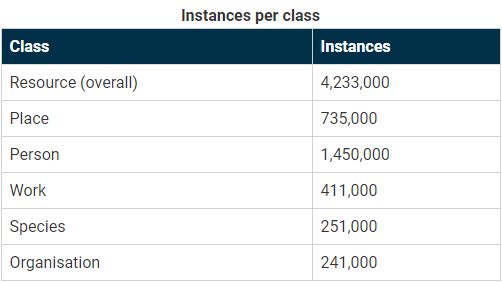
\includegraphics[width=.5\paperwidth]{dbpediaontology}
	\end{center}
	\caption{DBPedia Ontology instances per class \cite{dbpedia2019ontology}}
	\label{fig:ontology}
\end{figure}

The DBpedia extraction framework is responsible for extracting data from Wikipedia into a structured knowledge base, an overview of which is shown in Figure~\ref{fig:extraction}. This extraction is structured into four phases, as described by \citet{lehmann2015dbpedia}:

\begin{itemize}[label={},itemindent=-2em,leftmargin=2em]
	\item {\bf Input:} Wikipedia pages are read from an external source, either from a Wikipedia dump, or using the MediaWiki API.
	\item {\bf Parsing:} Each Wikipedia page is parsed, which transforms the source code of the Wikipedia page into an Abstract Syntax Tree (AST). An AST is a tree representation of the syntactic structure of the source code.
	\item {\bf Extraction:} The Abstract Syntax Tree of each page is forwarded to the extractors. There are many types of extractors, which will later be described, which extract data such as labels, images and infoboxes. Each extractor takes an AST as input and yields a set of Resource Description Framework (RDF) statements. These are XML statements which describe properties and values of resources.
	\item {\bf Output:} These RDF statements are written into sinks, which receive the data.
\end{itemize}

\begin{figure}[h]
	\begin{center}
		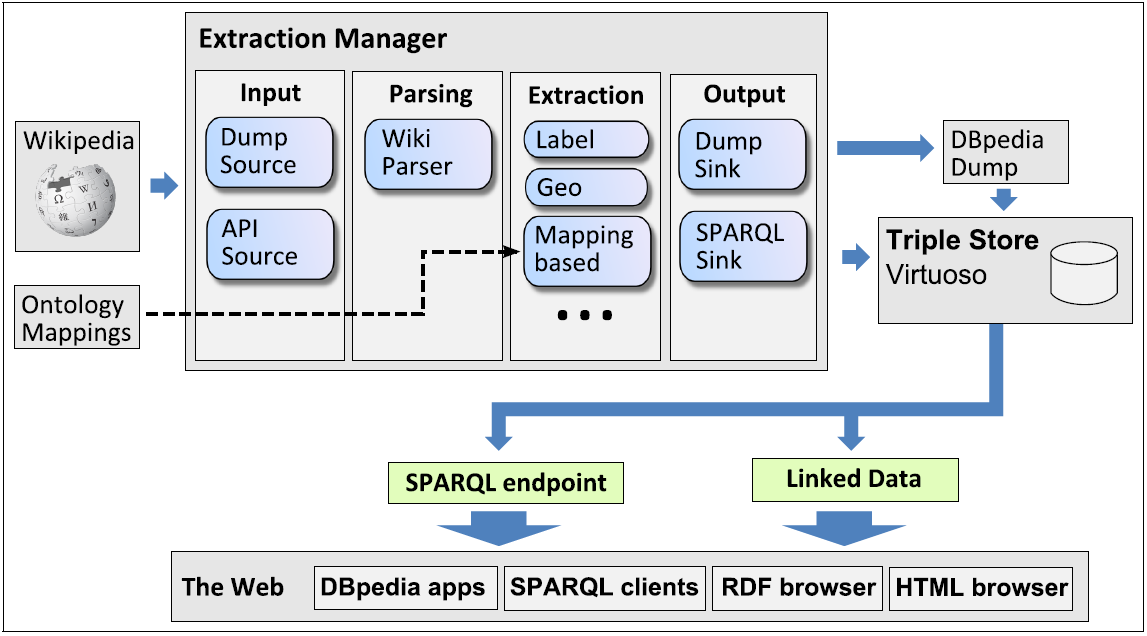
\includegraphics[width=.6\paperwidth]{dbpediaextraction}
	\end{center}
	\caption{DBpedia extraction framework \cite{bizer2009dbpedia}}
	\label{fig:extraction}
\end{figure}

The DBPedia ontology organises its entities using RDF models, each of which has many properties and are linked to subclasses and super-classes. This can be seen in Table~\ref{tab:ontology}, where a subclass may inherit the properties of its parent class. This can assist querying and searching, as we can query the data based on properties of a given class, as well as filtering with conditional queries. 

\begin{table}[h]
	\centering
	\begin{tabular}{{@{}lll@{}}}
		\toprule
		Ontology class & Instances & Example properties \\
		\midrule
		Person & 198,056 & name, birthdate, birthplace, employer, spouse \\
		\hspace{3mm} Artist & 54,262 & activeyears, awards, occupation, genre \\
		\hspace{6mm} Actor & 26,009 & academyaward, goldenglobeaward, activeyears \\
		\hspace{6mm} MusicalArtist & 19,535 & genre, instrument, label, voiceType, activeyears \\

		Athlete & 74,832 & currentTeam, currentPosition, currentNumber \\

		Politician & 12,874 & predecessor, successor, party \\
		\bottomrule
	\end{tabular}
	\caption{Example DBPedia classes and example instances \cite{lehmann2015dbpedia}}
	\label{tab:ontology}
\end{table}

The data extracted by the Extraction Manager is mapped to the ontology classes and properties to provide structured RDF statements. This allows instances of classes to be queried using the SPARQL query language \cite{sparql}, which returns data in the RDF format. The role of RDF is to provide semantics and structure to the information \cite{decker2000semantic}, which aligns with Tim Berners-Lee's vision of the next generation of the Web known as the Semantic Web \cite{berners2001semantic}. The DBPedia RDF Data Set is hosted and published using OpenLink Virtuoso, which provides a public SPARQL endpoint for querying the data \cite{lehmann2015dbpedia}; the RDF Dumps are also available to be downloaded in full.

The DBPedia data set is a strong candidate for use in this project because of its large scope and capacity for querying the data. The public SPARQL endpoint will also allow the dataset to be quickly investigated and tested.

\subsection{Other Candidates}
\label{subsec:candidates}
A widely used resource for data science and machine learning is Kaggle \cite{kaggle}, which is an online community that provides public and licensed datasets for use in data science projects and competitions. Previous works have used the resource to develop computer-aided diagnosis (CAD) systems for diagnosing cancers \cite{kuan2017deep}. More relevant to this project, \citet{uchendu2019characterizing} used the rDany dataset \cite{rdany} to distinguish between human and computer-generated messages. The Kaggle community is therefore a resource worth utilising for this project, and can provide data for further developments to the project in the future.

In the context of Wikipedia information, MediaWiki provides an API for retrieving and searching Wikipedia pages \cite{mediawiki}. While utilising this API would provide full access to the Wikipedia knowledge base, the data is not as manageable or queryable as that provided by the DBPedia resource. An example query response can be seen in Appendix~\ref{app:mediawiki}.

\newpage
\section{Programming Languages}
At its core, the language used to implement a chatbot has few criteria; it needs to be able to process natural language, provide a user interface for input and output, and can optionally interact with a data source. A bare minimum chatbot could therefore be implemented with virtually any programming language. However, it is important to consider the capabilities of the language, including support for machine learning, database interactions, and user interface design. This section will compare programming technologies based on their performance, their compatibility with the chatbot models previously discussed in the report, and the availability of libraries and functionality which may be useful for implementing a fully-featured, extensible chatbot.
 
\subsection{Python}
Python has been widely adopted in the scientific industry \cite{bird2009natural}, touted for its extensive collection of scientific libraries \cite{koepke2011python}; it recently eclipsed Java to become the most popular language, according to IEEE Spectrum \cite{cass2019}. Natural language processing can be quickly implemented with libraries such as Natural Language Toolkit (NLTK) \cite{nltk2019}; artificial neural networks (ANNs) can be leveraged with many libraries, including Scikit-learn \cite{pedregosa2011scikit}. Newer developments in machine learning include TensorFlow \cite{abadi2016tensorflow}, which provides a novel learning framework utilised in large-scale machine learning applications such as healthcare \cite{polzin2019} and Google’s own search engine \cite{pichai2015}. In the context of chatbots, Python allows for interpretation of AIML with the python-aiml library \cite{villegas2019}; more comprehensive chatbot libraries can also be utilised, such as ChatterBot \cite{cox2019}. Using Python would therefore provide the freedom to explore various technologies for implementing the project and extend the functionality in the future, given the abundance of relevant libraries.

In terms of linking data sources, the database access layer in Python is inherently weaker than other technologies such as JDBC and ODBC \cite{vermuelen2019}. However, this is mainly a concern for enterprise solutions, as Python’s DB-API specification can connect to most databases \cite{python2017db}. Furthermore, connecting to a SPARQL endpoint and parsing RDF graphs is possible through RDFLib \cite{rdf2019}. Many Python web frameworks can handle user interaction, routing, and security. Some of the popular web frameworks include Django, TurboGears, and Flask \cite{python2020web}. These frameworks vary in their features, but for the scope of this project, it is safe to assume that any of them will fit the criteria and they can be explored further in the experimentation phase.

Python has been used extensively in the machine learning field, and can be seen in many Machine Learning as a Service (MLaas) services; the Microsoft Azure Machine Learning service uses Python for training and modelling \cite{microsoft2019architecture}. Python would be an effective language to use to implement a project of this scope.

\subsection{Java}
Java is widely used in machine learning implementations \cite{witten2005practical, abeel2009java}, and is prevalent in research and enterprise solutions. Many libraries exist to implement machine learning frameworks \cite{kovalev2016deep}, natural language processing \cite{nltk2019}, and AIML interpreters \cite{alice2013}. Java has the advantage of being natively cross-platform since the Java program is compiled into byte-code to be interpreted by the Java virtual machine (JVM) \cite{witten2005practical}; this may beneficial to this project if it is deployed to a Linux web server.

Querying and interpreting RDF data can be achieved using Apache Jena \cite{apachejena}, and dependency management can be facilitated using several tools such as Apache Maven \cite{apachemaven} and Gradle \cite{gradle}. Many web frameworks exist in order to manage web requests, such as Spring \cite{springmanual} and JavaServer Faces \cite{mcclanahan2004javaserver}. Java has been established as being performant and scalable in general-use programming \cite{moreira2000java}, and the JVM is leveraged by other languages such as Scala \cite{odersky2008programming}. Therefore, implementing the project using Java would provide access to a vast array of libraries and frameworks, and allow for further expansion in the future.

\subsection{Alternatives}
Given the diverse landscape of programming languages available, it is worthwhile to consider how related works are implemented. The original implementation of ALICE by \citet{wallace2009anatomy} was originally programmed in Lisp \cite{winston1986lisp}. Since then, Clojure, a Lisp 'dialect' that runs in the JVM \cite{hickey2008clojure}, has been widely used in machine learning \cite{wali2014clojure}, and can easily take advantage of concurrency in multicore and distributed systems \cite{emerick2012clojure}. Similarly, Scala, another JVM language used in data-driven programming \cite{wampler2014programming}, is employed by the DBPedia Lookup project for searching and ranking DBPedia resources by keyword \cite{dbpedialookup}.

Ruby on Rails (RoR) is a web application framework used widely on the Web \cite{paplauskaite2016}. Web applications using this framework benefit from the RoR principles of 'Convention over Configuration' CoC and 'Don't Repeat Yourself' \cite{bachle2007ruby}, which accelerate development of applications. This framework was used effectively by \citet{horzyk2009intelligent} to create a chatbot shop-assistant that adapts to a customer's perceived personality.

\subsection{Conclusion}
Having explored a number of programming languages, it is evident that a project of this scope could be implemented in any of the languages explored above, and many more, due to the availability of relevant libraries. The choice of programming language used for the project will be further explored and justified in Section~\ref{sec:lang}.

\cleardoublepage
\section{Existing Solutions}
\label{sec:existing}
Dialogue systems are abundant in business and consumer use, from ordering pizza with a Google Home device \cite{google2018dominos}, to diagnosing and managing patients’ medical conditions \cite{yourmd2017}. This section will explore existing solutions that are relevant to the scope of this project, as well as broader chat systems currently in use.

\subsection{Google Assistant}
Google Assistant is a popular and highly available intelligent virtual assistant (IVA) offering from Google \cite{lopez2017alexa}. It provides a vast array of functions, such as searching and integration with enabled `smart devices' \cite{googleassistant}. Google Assistant also incorporates other Google services, including search, which facilitates keyword queries about almost any topic \cite{michaely2017keyword}, as seen in Figure~\ref{fig:assistant}.

One standout feature of Google Assistant is its contextual understanding, which Google brands as Continued Conversation \cite{paplauskaite2016}. As concluded by \citet{tulshan2019survey}, Google Assistant is the most effective IVA at contextual understanding, which is demonstrated in Figure~\ref{fig:assistant}.

It is clear that the functionality of Google Assistant eclipses the scope of this project. However, there are several features from which this project can draw inspiration. For example, contextual understanding would be an effective feature to integrate into the chatbot to make conversational queries more efficient. The drawback of Google Assistant is its propietary nature, meaning that we cannot investigate how it is implemented, nor can we extend it in this project.

\begin{figure}[h]
	\centering
    \subfloat[Querying Google Assistant]{{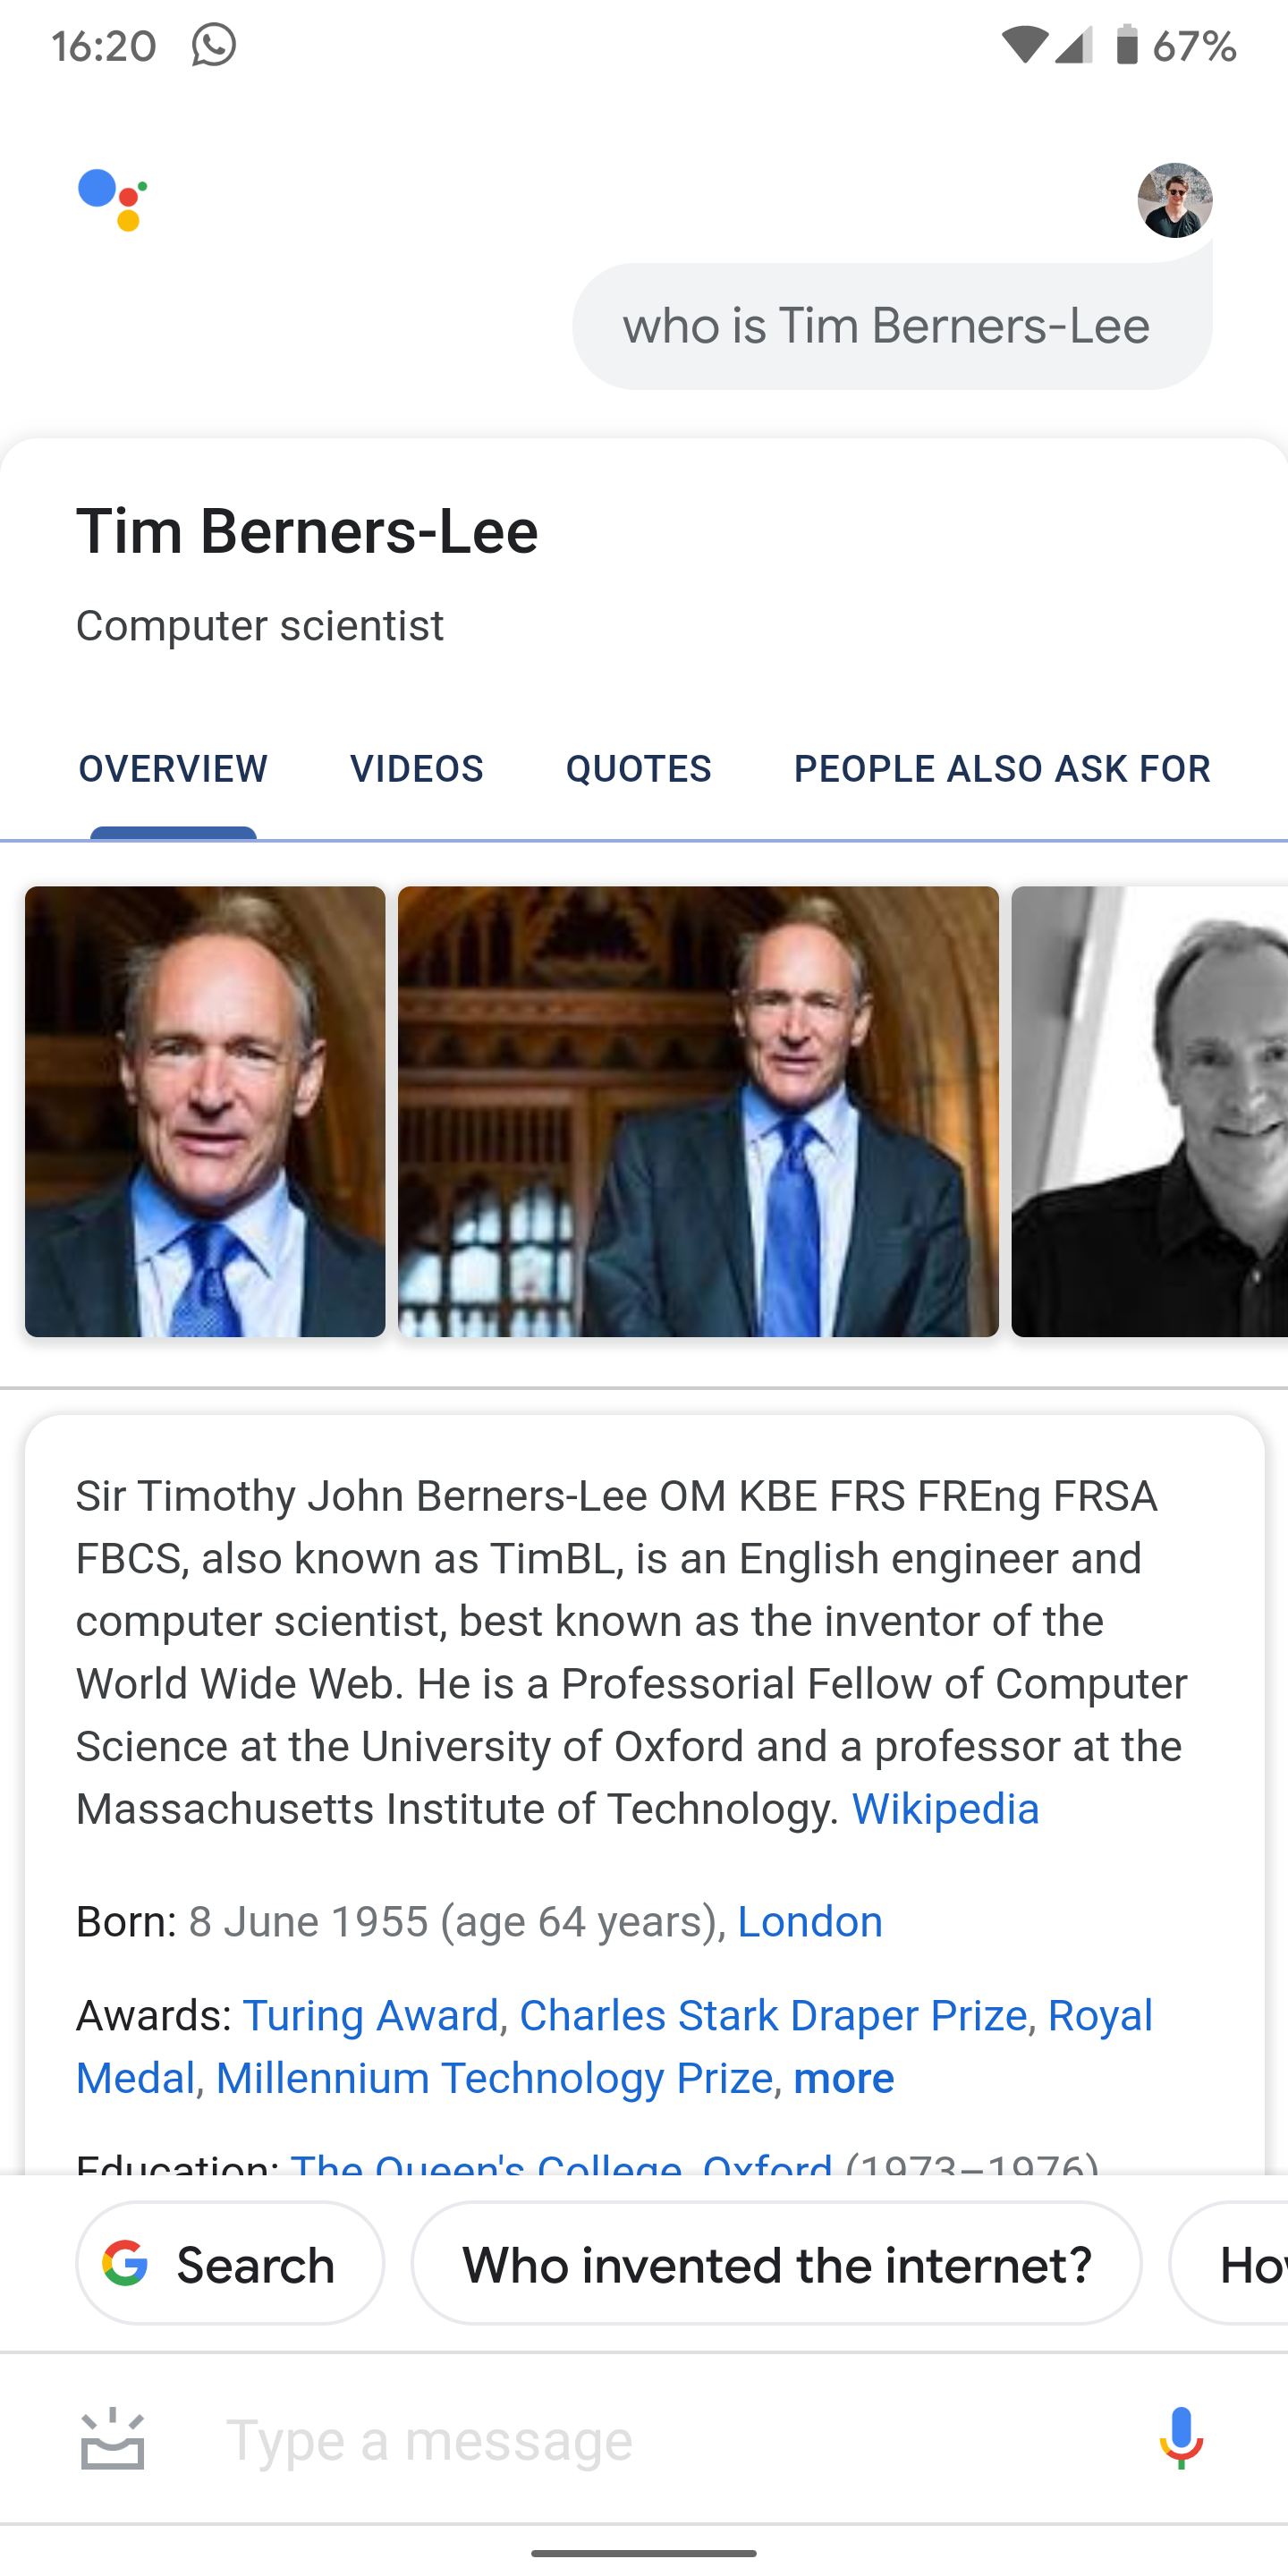
\includegraphics[width=5cm]{assistant1} }}%
    \qquad
	\subfloat[Google Assistant's Continued Conversation]{{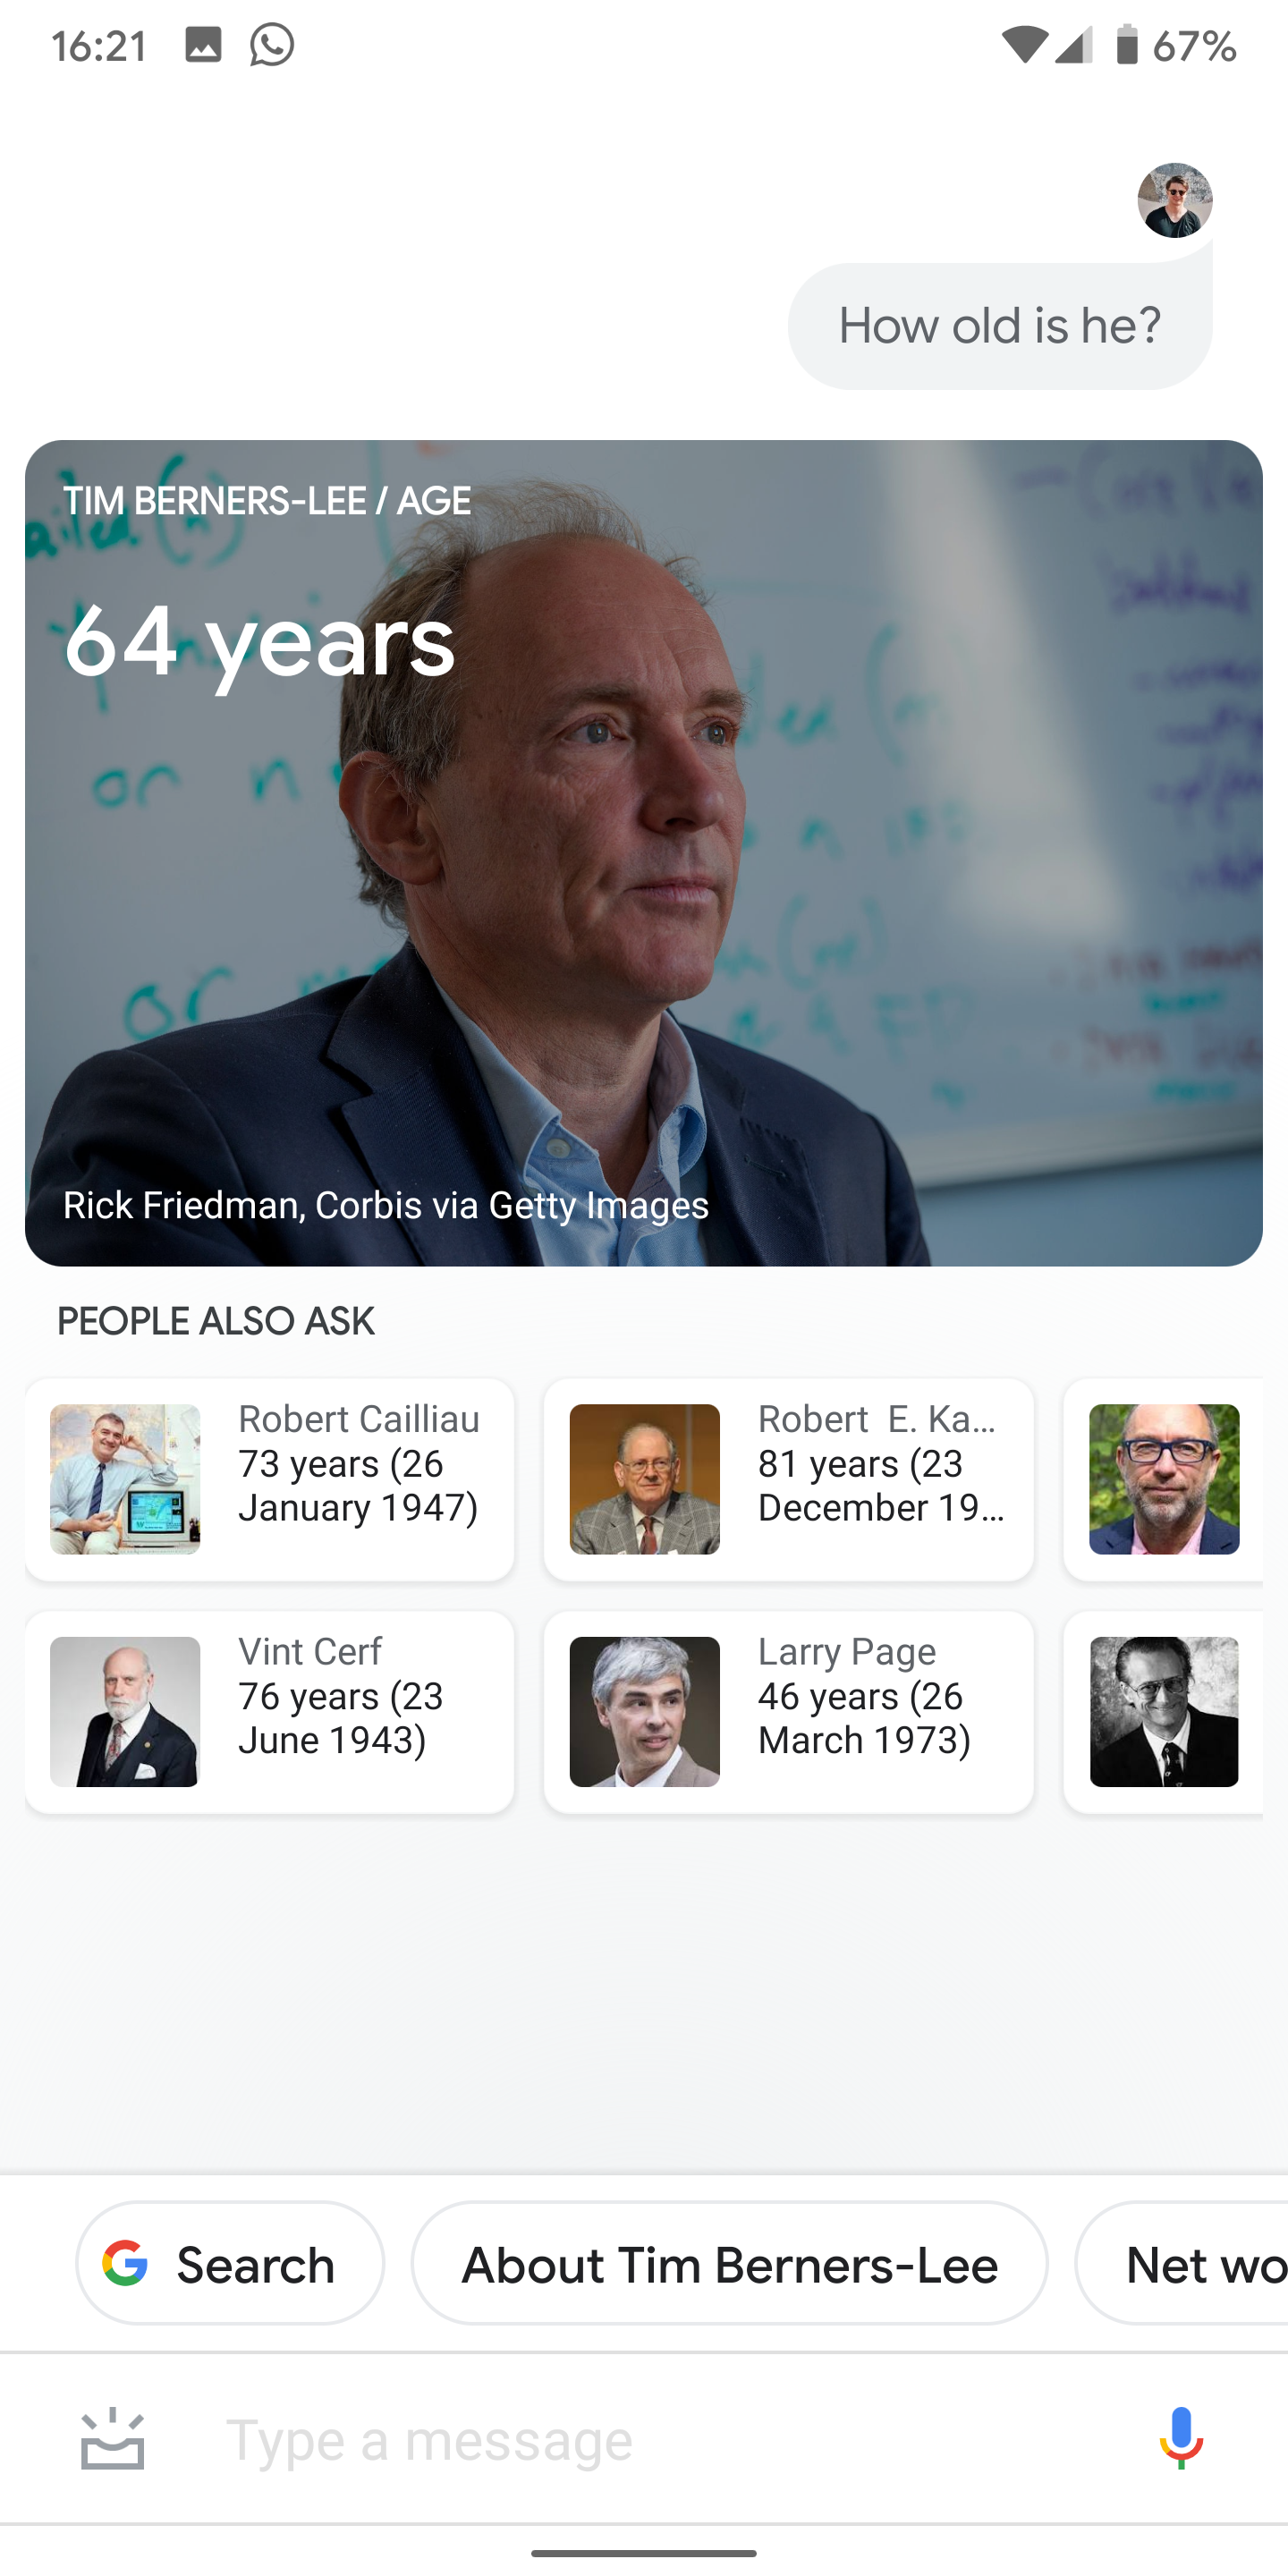
\includegraphics[width=5cm]{assistant2} }}%	
	\caption{A conversation with Google Assistant}
	\label{fig:assistant}
\end{figure}

\newpage
\subsection{DBPedia Chatbot}
\label{sec:dbchatbot}
The system that resembles the scope of this project closest is DBPedia Chatbot \cite{ramngongausbeck2018}. The project integrates with the DBPedia dataset to provide a chatbot which allows users to pose questions, and the system then generates a response using information from the dataset.

Upon investigating the solution, the chatbot can only interpret a small set of predetermined queries. When a query outside of this question set is posed, the chatbot throws an error -- as shown in Figure~\ref{fig:dbchatbot}. This could either be a limitation of the implementation itself, or the publicly available demo website \footnote{http://chat.dbpedia.org/}. Therefore, this project can expand beyond the scope of the implementation provided by \citet{ramngongausbeck2018}, including more advanced queries and filtering. The rich response elements seen in Figure~\ref{fig:dbchatbot} are effective and this project can draw inspiration from them in the final implementation.

\begin{figure}[h]
	\centering
	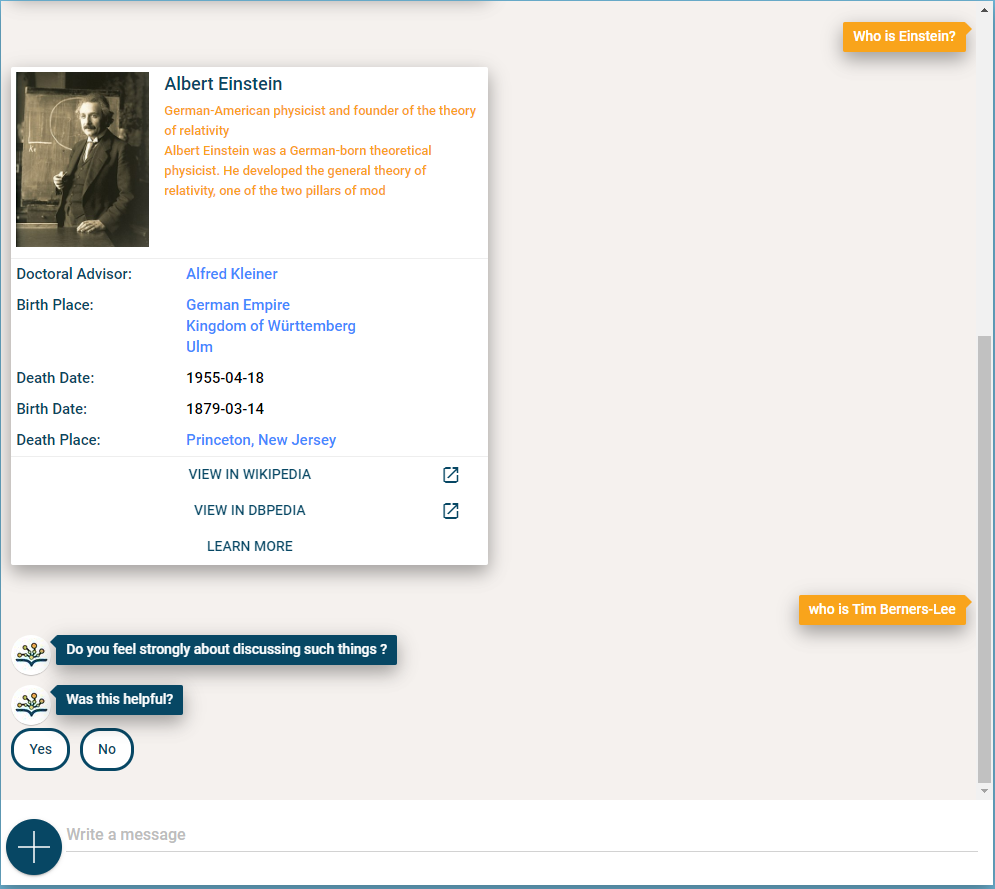
\includegraphics[width=.5\paperwidth]{dbchatbot}
	\caption{DBPedia Chatbot implementation \cite{ramngongausbeck2018}}
	\label{fig:dbchatbot}
\end{figure}

\newpage
\subsection{Mitsuku}
\label{subsec:Mitsuku}
Mitsuku is a chatbot implementation created by Steve Worswick \cite{worswick2018mitsuku} which has won the Loebner Prize a record five times \cite{aisb2019}. The chatbot is implemented using AIML \cite{higashinaka2014towards}, and is designed to handle open conversation with Mitsuku, who claims to be an eighteen year-old girl \cite{abdul2015survey}.

Mitsuku deals well with general conversation and banter, and responds in a humourous and intelligent manner. As can be seen in my dialogue with her in Appendix~\ref{app:mitsuku}, this implementation is effective at establishing a distinct and discernible personality for Mitsuku. Although Mitsuku only seems to handle a set of predetermined queries (see Figure~\ref{fig:mitsuku}), it is clear that the purpose of Mitsuku is not to serve as a knowledge base, but as a general-purpose conversational bot. She handles open questions intelligently, and seems to have a large repository of conversation topics and responses. She also manages multi-turn dialogues well, and is effective at maintaining the context of the conversation. Mitsuku is closed-source, so the AIML definitions cannot be explored, but this project can take inspiration from the conversation style of Mitsuku.

\begin{figure}[h]
	\centering
	\subfloat[Querying Mitsuku]{{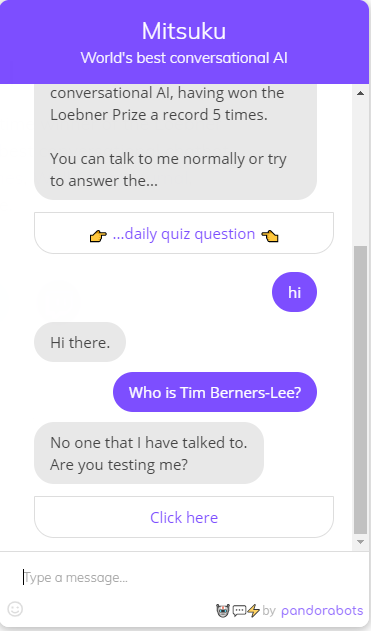
\includegraphics[width=5cm]{mitsuku1} }}%
	\qquad
	\subfloat[Mitsuku known result]{{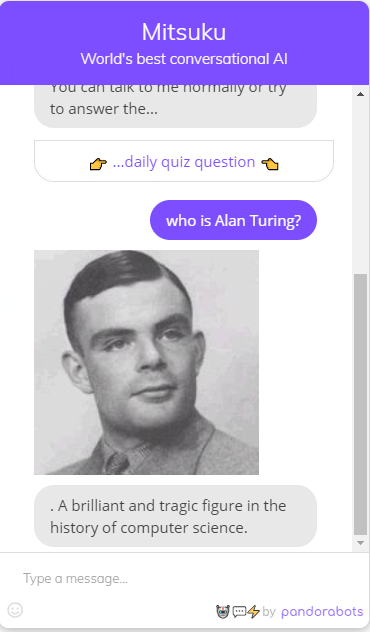
\includegraphics[width=5cm]{mitsuku2} }}%	
	\caption{A conversation with Mitsuku}
	\label{fig:mitsuku}
\end{figure}

%\subsection{DBPedia Spotlight}

\newpage
\section{Related Work}
Chatbot designs have been thoroughly investigated by \citet{abdul2015survey}, who conclude that there does not yet exist a common chatbot approach, although pattern matching techniques such as AIML are effective in closed-domain systems. It is, however, a field that is seeing frequent and significant developments from researchers and companies.

\citet{yan2016learning} found that a neural network approach, known as {\it deep learning-to-respond}, outperforms pattern-matching and retrieval-based models in open-domain generative systems. Similarly, \citet{mikolov2011extensions} concludes that recurrent neural network language models are the most effective technique in linguistic tasks such as machine translation and automatic speech recognition.

As examined in Section~\ref{sec:dbchatbot}, \citet{ramngongausbeck2018} implemented a chatbot using DBPedia as a datasource. This work can be extended in the scope of this project, by providing a complete and more advanced system. \citet{bradevsko2012survey} observed a trend in chatbot systems towards {\it semantics}, which will be further explored in this project.

\section{Conclusion}
This review has explored chatbots and how they are currently being used in industry and research. We are seeing a trend towards chatbots being used in many businesses, from customer service to healthcare; the fields of human-computer interaction and machine learning are seeing many new and significant developments. Chatbot systems are becoming prevalent in modern life, so exploring this evolution will be one of the main objectives of this project.

As the Web trends towards the new era of the Semantic Web, methods of extracting and interpreting information are evolving. Developing a chatbot to understand semantic data will form a basis for future developments and extensions of this project.

The next step for this project is to design a chatbot solution based on the outcome of the research. As is evident from the existing solutions that have been explored, a chatbot can be implemented with an array of available technologies. The next sections of this report will consider how these technologies can be implemented to develop a novel and successful chatbot solution that fits the requirements determined in the analysis phase.






	\chapter{Analysis}
\label{ch:analysis}
\section{Introduction}
Following the structure of the Software Development Life Cycle (SDLC) \cite{sdlc2010}, the analysis section ensures that the proposed application meets the requirements of the end user. Once the requirements are gathered, a list of requirements is proposed and accepted by the end users, and the requirements are prioritised according to how important each is for the user to meet a minimum functional system.

\section{Requirements Gathering}
In order to build a successful solution, the requirements of the system are first gathered. This begins with assessing current solutions and related works to establish what makes them successful, as well as identifying any shortcomings in these solutions. I then communicate with the end users, to determine the features the chatbot system should have.

\subsection{Research}
In Section~\ref{sec:existing}, we identified a number of existing chatbot systems which relate to the proposed solution. These include Google Assistant, Mitsuku, and an existing DBPedia chatbot implementation.
\hilight{continue}

\subsection{Users}
For this project, I enlisted three end users to aid the development and testing of this proposed system. Two of these users are colleagues of mine on my course, and one is an outside user with less technical knowledge.
\hilight{continue}

\newpage
\section{System Requirements}
\label{sec:requirements}
This section defines the functional and non-functional requirements the system must meet. This specification was produced in collaboration with the three test users across a number of conversations with them. We also determined how important each requirement is, and a breakdown of the priorities will be analysed in Section~\ref{sec:priority}.

\subsection{Functional Requirements}

\begin{itemize}
	\item User Interaction
	\begin{enumerate}[label*=F\arabic*.]
		\item User Interaction - The application should allow the user to interact with the chat bot
		\item Browser Access - The user should be able to access the chatbot in a browser
		\item Text Input - The user should have a text box to type their query
		\item Responses on Page - The user should clearly see the response of the chatbot in the webpage
		\item Conversation History - The user should be able to clearly see their conversation history with the chatbot in the webpage
	\end{enumerate}
	\item Basic Queries
	\begin{itemize}
		\item The chatbot can answer basic questions about Person articles
		\begin{enumerate}[resume*]
			\item Person Description Query - The application should take a user query about a person - ‘who is X’ - and respond with a description of that person.
			\item Person Birthdate Query - The application should take a user query about the birthdate of a person – ‘when was X born’ and return the birthday of the given person.
			\item Person Age Query - The application should take a user query about the age of a person - ‘how old is X’ - and return the age of the given person.
			\item Person Birthplace Query -The application should take a user query about the birth place of a person – ‘where was X born’ -  and return the birth place of the given person. 
			\item Person Death Date Query - The application should take a user query about the death date of a person – ‘when did X die’ and return the birth place of the given person. 
			\item Person Known For Query - The application should take a user query about what a person is known for – ‘what is X known for’ and return a description of what the given person is known for.
			\item Person Photo Query - The application should take a user query about what a person looks like – ‘photo of X’ or ‘what does X look like’ - and return a photo of the person
			\item Person Wikipedia Link Query - The application should take a user query about linking to the Wikipedia page of a person, and return a link to that page.
		\end{enumerate}
		\item The chatbot can answer questions about countries
		\begin{enumerate}[resume*]
			\item Country Description Query - The application should take a query about a country, and return the description of that given country.
			\item Country Population Query - The application should take a query about the population of a country, and return the population of that given country.
			\item Country Capital Query - The application should take a query about the capital of a country, and return the capital of the country.
			
		\end{enumerate}
	\end{itemize}
	\item Advanced Queries
	\begin{itemize}
		\item The chatbot can answer advanced queries about Person articles:
		\begin{enumerate}[resume*]
			\item Person List Query - The user should be able to find a list of people who meet a certain criteria. \\
			e.g. ``People born in 1980'' or ``List of actors born in London''
			\item Person AND Query - The user should be able to combine queries using ‘AND’ to find people who satisfy two conditions. \\For example, "People who were born in 1980 AND were born in London"
			\item Context-aware Conversation - The user should be able to ask sequential queries about a topic and the chatbot will be able to answer queries within that context. \\ For example, the user first asks ‘Where was X born’, the chatbot responds, and the user asks a follow up question ‘What about Y?’. The chatbot will then respond to the second query with an answer that satisfies the query ‘where was Y born’.
		\end{enumerate}
	\end{itemize}
	\item Conversation
	\begin{enumerate}[resume*]
		\item Chatbot Greeting - The user should greet the chat bot and be returned with a similar greeting – e.g. Hello.
		\item Chatbot Examples - The user should be able to ask for example queries and the chat bot returns a number of working example queries
		\item Chatbot Help - The user should be able to ask for help using the chatbot and be returned with a statement about how to use the chat bot.
	\end{enumerate}
\end{itemize}

\subsection{Performance Requirements}
\begin{itemize}
	\item Performance
	\begin{enumerate}[label*=P\arabic*.]
		\item The web page should load fully in less than 5 seconds
		\item The chat bot should respond to each query within 5 seconds
	\end{enumerate}
	\item Reliability
	\begin{enumerate}[resume*]
		\item The application should function without failure
		\item Any errors that do occur during normal operation should be logged, and the user should be clearly informed that an error has occurred.
	\end{enumerate}
\end{itemize}

\section{Requirement Prioritisation}
\label{sec:priority}
In order to meet the deadline of the project, some features may not be implemented. To prepare for this, it is important to define which requirements are the highest priority for the chatbot, and which could be considered optional and implemented in the future. To do this, I met with my three testers to discuss how the requirements should be prioritised. Table~\ref{tab:priority} outlines the priority of each requirement, as well as some notes or justification that was posited in this discussion.

\begin{table}[h!]
	\centering
	\begin{tabularx}{\textwidth}{{@{}lcX@{}}}
		\toprule
		Requirement & Priority & Justification \\
		\midrule
		F1.  User Interaction & High & User has to interact with chatbot. \\
		F2.  Browser Access & High & Browser more user-friendly than command-line. \\
		F3.  Text Input & High & Required for user interaction. \\
		F4.  Responses on Page & High & Required for user interaction. \\
		F5.  Conversation History & High & Useful for having multi-line interaction with bot. \\
		F6.  Person Description Query & High & Useful to get information about given person. \\
		F7.  Person Birthdate Query & High & Probably a highly requested query. \\
		F8.  Person Age Query & Medium & Useful to find out quickly a person's age. \\
		F9.  Person Birthplace Query & Medium & May be useful when finding many people from the same place. \\
		F10. Person Death Date Query  & Low & Could be helpful for historical figures. \\
		F11. Person Known For Query & Medium & A useful query for scientists and historical figures. \\
		F12. Person Photo Query & Medium & Helpful to have a visual reference for a person. \\
		F13. Person Wikipedia Link Query & Medium & User would be able to find out more about the given person. \\
		F14. Country Description Query & Low & Testers were unsure whether a description of a country is useful. They would probably use it more for facts and figures. \\
		F15. Country Population Query & Medium & This statistic may be useful for comparing countries. \\
		F16. Country Capital Query & High & Testers said this would likely be the most sought-after information. \\
		F17. Person List Query & Medium & Provides unique functionality for the user \\
		F18. Person AND Query & Low & Could be useful for more advanced searches. \\
		F19. Context-aware Conversation & Medium & Helpful for usability of bot, could be a standout feature for system. \\
		F20. Chatbot Greeting & Medium & Helps with `friendliness' of bot. \\
		F21. Chatbot Examples & High & Useful to know what the users could ask. \\
		F22. Chatbot Help & High & Helpful if users get stuck or are using the system for the first time. \\
		
	\end{tabularx}
	\caption{Software requirements prioritisation.}
	\label{tab:priority}
\end{table}

\newpage
\section{Project Scope}
\label{sec:scope}
As conversations with chatbots can be open-ended, it will be necessary to restrict the scope of the project to the requirements specified in Section~\ref{sec:requirements}. While it may be tempting to add a variety of features and conversation topics with the chatbot, a successful result will be that the requirements of the system are met and can be successfully validated.

One of the main aims of the project from Section~\ref{sec:aims} was to develop a successful system that can be expanded in the future. Based on the current requirements, it is feasible that future extensions to the project will be possible, based on the system implemented in this stage of the project.

\section{Summary}
This chapter has determined the requirements of the proposed system, as well as how those requirements will be met by a successful implementation. While the initial system may be basic, the project will be further extensible in the future. The next chapter will outline the design of the proposed chatbot.
	\chapter{Design}
\section{Methodology}
\section{Architecture}
\section{User Interface}
\section{Experimentation}
	\chapter{Implementation}
\label{ch:implementation}
\section{Introduction}
This chapter describes the planning and implementation phases.

\section{Software Development Methodology}
\subsection{Waterfall Model}
\subsection{}

\section{Planning}
As the timeline of the project is restricted and has a fixed deadline, it is important that the project is planned carefully in order to deliver a complete solution.

Gantt


\section{Version Control}
Git - branches

\section{Dependency Management}

\section{Implementation Process}
Following the Gantt chart, ...

\subsection{Initialisation}
The first step of the implementation was to initialise a Git repository and a Java environment with Maven dependency management. Since the project would depend on many libraries for displaying and processing data, Maven is able to manage versioning and interdependencies of these libraries.

\subsection{Program AB}
As a result of the research in earlier phases, it was decided that this system would use a rule-based chatbot architecture, namely AIML as it is widely used in current chatbot systems. Program AB is a Java implementation of AIML 2.0 provided by ALICE A.I. Foundation \cite{programab_2013}. While this repository is no longer being developed, the choice for this project was to use a fork of this source, which is provided as a Maven dependency \cite{lumenrobot2016}.

Once the Maven dependency had been loaded into the project's \code{pom.xml} file, I was able to experiment with the chatbot. The \code{program-ab} source contains the original AIML implementation of a bot named S.U.P.E.R. created by \citet{wallace2009anatomy}, which gives examples of the many elements of the AIML style.

An initial program was written for experimenting with AIML and the example bot, as seen in Figure~\ref{fig:super}. 

\begin{figure}[ht]
	\centering
	\subfloat[Initial code]{{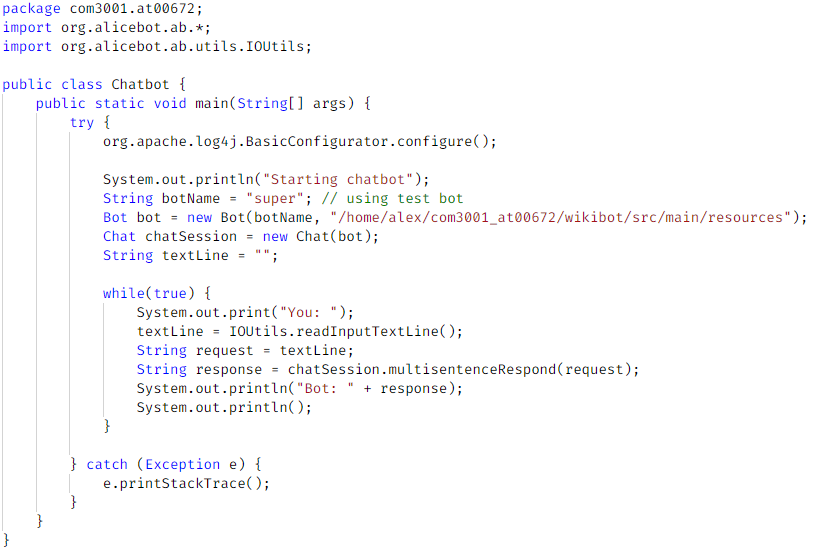
\includegraphics[width=12cm]{code1} }}%
	\qquad
	\subfloat[Chatting with S.U.P.E.R.]{{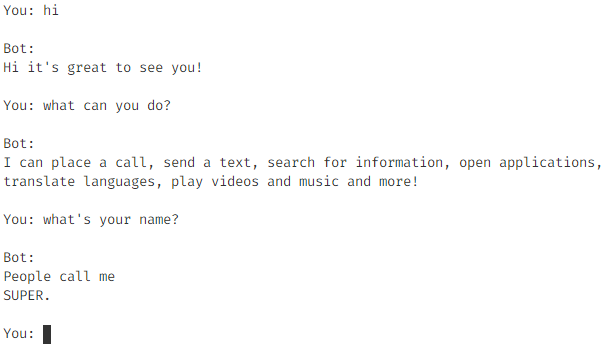
\includegraphics[width=12cm]{super} }}%	
	\caption{Initial chatbot interactions}
	\label{fig:super}
\end{figure}

\newpage
Having experimented with the example chatbot, my next task was to initialise my own chatbot. The Program AB Bot has a number of functions to load its required files from a directory. The file structure is as follows:

\begin{outline}
	\1 \textbf{bots} The parent bots directory
		\2 \textbf{\emph{botName}} The name of the bot
			\3 \textbf{aiml} The AIML pattern files 
			\3 \textbf{aimlif} AIML Intermediate Format files which are generated by the Bot
			\3 \textbf{config} Configuration files
			\3 \textbf{maps} Map files
			\3 \textbf{sets} Set files
\end{outline}
	
Once the structure was initialised, a file was created named \code{conversation.aiml}, which contained the first AIML patterns for conversing with the chatbot. The contents of this file are shown in Figure~\ref{fig:aiml1}. Some of the key features here are the use for the \code{<srai>} tag on line 17, which is a powerful function for resolving synonyms here. This allows us to route the input of `hi' to the `hello' pattern. This saves us repeating several lines of code, and is used heavily later in the project. Also, in lines 4 and 15 we are using wildcard symbols. This allows us to match zero or more words, and these can then be passed into other parts of the conversation. In AIML, the following wildcards can be used:

\begin{itemize}
	\item \# matches zero or more words (higher priority)
	\item \_ matches one or more words (higher priority)
	\item \^{} matches zero or more words (lower priority)
	\item * matches one or more words (lower priority)
\end{itemize}

So in our `hello' example, the given pattern will match any of the following inputs: {\it{`Hello', `Hello there', `Hi bot', `Hi', `Hi there'}}. It will not, however, match an input such as {\it{`Why hello there'}}, because we have not told the bot how to divide that given input; nor does the bot recognise {\it{`good afternoon'}} and so on.

\begin{figure}[h]
	\centering
	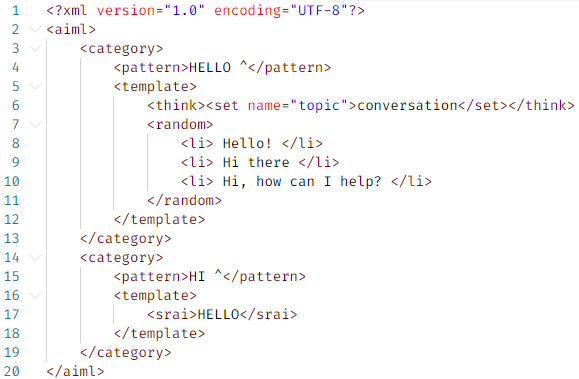
\includegraphics[width=.5\paperwidth]{aiml1}
	\caption{Initial AIML configuration}
	\label{fig:aiml1}
\end{figure}

\newpage
\subsection{DBPedia}
Now that the basic chatbot system has been set up, we need to provide functionality to the system by querying our datasource. DBPedia was selected based on the research in Section~\ref{sec:dbpedia}, because it provides an organised dataset from Wikipedia articles. It can be queried via a SPARQL endpoint, and returns data in an RDF format, which can be processed by our system.

There are a number of online resources which allow us to experiment with querying DBPedia. My preferred resource is SPARQL Explorer \footnote{http://dbpedia.org/snorql/}, which allows us to write queries and see the result in several formats, including a tabular format. For example, if we want to find musicians born in Manchester, we can construct the following SPARQL query:
\begin{figure}[h]
	\begin{lstlisting}
		SELECT ?person ?birthPlace ?name
		WHERE {
		  ?person a dbo:MusicalArtist .
		  ?person rdfs:label ?name .
		  ?person dbo:birthPlace ?birthPlace .
		  filter(?birthPlace = dbr:Manchester)
		  filter(langMatches(lang(?name), 'en'))
		} LIMIT 50 
	\end{lstlisting}
	\caption{An example SPARQL query}
	\label{fig:sparql1}
\end{figure}

Executing this query returns a list of the first 50 results of musicians born in Manchester, as shown in Figure~\ref{fig:sparql1}. The format of SPARQL queries has some similarities with SQL queries, using keywords such as \code{SELECT} and \code{WHERE}. In this query, we are filtering to find each person that has the property \code{dbo:MusicalArtist}, which is shorthand for \url{http://dbpedia.org/ontology/MusicalArtist}, referencing the DBPedia ontology. We are setting the variable \code{?name} to the property \code{rdfs:label} which contains the name attribute of the person; the same applies for \code{dbo:birthPlace} referencing their birth place. Finally, we are filtering the results; we want the results to only contain musicians whose birth place is Manchester; next we filter the \code{?name} results by language, to remove any duplicate results where the name is given in multiple languages.

\begin{figure}[h]
	\centering
	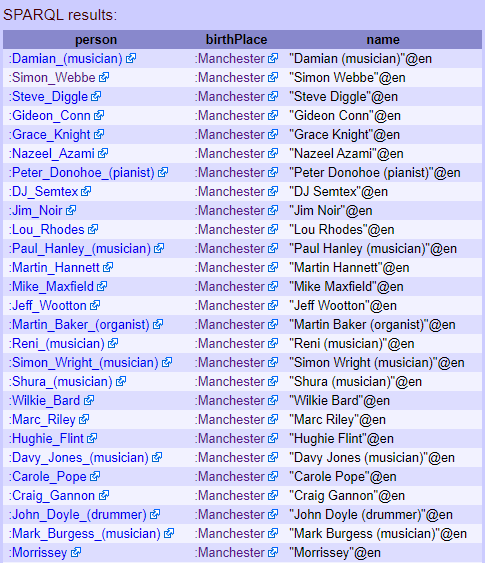
\includegraphics[width=8cm]{snorql}
	\caption{SPARQL query results}
	\label{fig:sparql2}
\end{figure}

In our Java system, these queries have to be constructed and executed programmatically, based on the user's input. For executing SPARQL queries, Apache Jena \cite{apachejena} provides RDF functionality for querying an RDF model. To test this, the Apache Jena dependencies are loaded into our Maven dependency file. This allows us to utilise the \code{org.apache.jena} libraries to query the endpoint. To test the connection, a function was written to test the DBPedia endpoint, as shown in Figure~\ref{fig:testrdf}.

\begin{figure}[h]
	\centering
	\subfloat[Test connection code]{{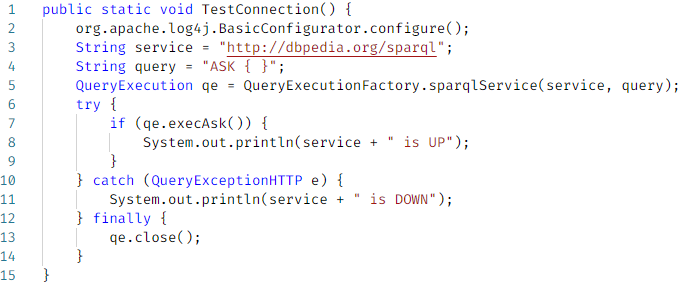
\includegraphics[width=.45\textwidth]{testrdf} }}%
	\qquad
	\subfloat[Successful result]{{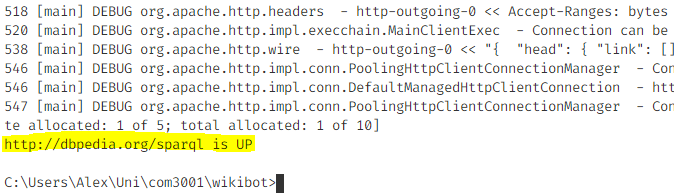
\includegraphics[width=.45\textwidth]{testrdf2} }}%
	\caption{Testing the SPARQL Endpoint}
	\label{fig:testrdf}
\end{figure}

For executing and processing more functional queries, we have to first generate a query string. As an example, we will use the query we saw in Figure~\ref{fig:sparql1}. Once the query has been executed, we have to loop through the results and do some processing, such as printing to the console. The process for this is shown in Figure~\ref{fig:querysparql}. Here, our query string requires the \code{PREFIX} keyword to define the names of the prefixes for the ontologies we are using. The result from this execution exactly matches the result from the experimentation in Figure~\ref{fig:sparql2}.

\begin{figure}[h]
	\centering
	\subfloat[Testing query code]{{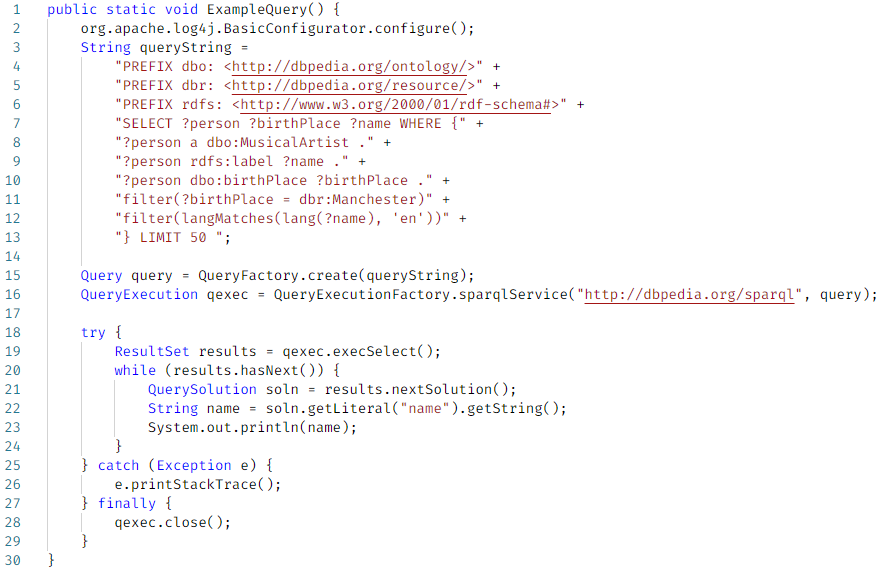
\includegraphics[width=.70\textwidth]{sparql1} }}%
	\qquad
	\subfloat[Result]{{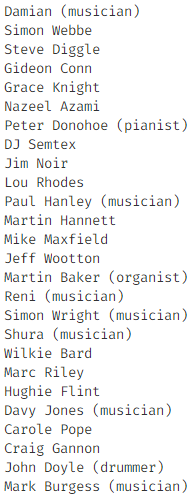
\includegraphics[width=.20\textwidth]{sparql2} }}%
	\caption{Querying the SPARQL endpoint}
	\label{fig:querysparql}
\end{figure}

\subsection{Linking the Chatbot}
Now that we have a basis for querying the DBPedia dataset, the chatbot now has to be able to query the endpoint. For this we need to implement the following:
\begin{enumerate}
	\item AIML patterns to match user input to a query
	\item A query builder to convert the user input into a SPARQL query
	\item A service to execute the function and process the results
\end{enumerate}
These functions align with the system architecture design seen previously in Section~\ref{sec:systemdesign}. The next sections explain how these were implemented and connected in the final system to achieve the required functionality.

\subsubsection{AIML Patterns}
One of the key functions of this chatbot is to match input patterns to desired queries. There are a number of challenges that arise here. Firstly, a query can be asked in many different ways. For example, to find out the date of birth of a person, a user may ask: {\it`What is *s birthdate?', `When was * born?', `* birth date', `Tell me when * was born'}. The bot must then distinguish between these queries and {\it`how old is *'} as those are two distinct functions.

Furthermore, one of the requirements of the system is that is can deal with pronouns and maintain context. As such, the user should be able to ask follow-up questions by continuing a conversation, e.g. {\it `When was he born?'} - the chatbot must remember who {\it `he'} is, and if that is not known, the chatbot must ask for more information to continue the query.

As such, the AIML patterns become more complex as the system develops to include more functions. For example, Figure~\ref{fig:aiml-comment} shows a fragment of the code for giving a description of a person (Requirement F6). The template uses a number of key features of AIML to achieve the desired functionality.
First, the wildcard (*) is used to match the user's input into the query. Next, the \code{<think>} allows us to programatically set the {\it{predicates}} of the conversation, which act in essence as variables that can be set and retrieved throughout the conversation. These predicates are sent to the \code{ChatbotService} module to process them into a meaningful result.

Line 14 redirects to \code{BOT\_QUERY\_CONTEXT}, the logic for which is shown in Figure~\ref{subfig:aiml1}.
This template determines whether or not a pronoun has been used - {\it{`Who is Alan Turing?'}} versus {\it{`When was he born?'}}. Line 5 uses the \code{<map>} function. Maps can be used to link an input to a result. In this example, our bot has a file named \code{pronouns.txt} in the \code{maps} folder of the bot resources, the contents of which is shown in Figure~\ref{fig:pronouns}. The map simply maps all pronouns to \code{they}. This means that if any pronoun was used, we determine this conditionally, as in Line 9. If the value of \code{subject} is \code{they}, we then check if the context has been set. If it has, we run the query using the subject that has been previously set. If not, we then ask the user for more information by redirecting to the template shown in Figure~\ref{subfig:aiml2}.

\begin{figure}[h]
	\centering
	\begin{lstlisting}
	he:they
	she:they
	him:they
	her:they
	they:they
	their:they
	\end{lstlisting}
	\caption{Contents of \code{pronouns.txt}}
	\label{fig:pronouns}
\end{figure}

\begin{figure}[pt]
	\centering
	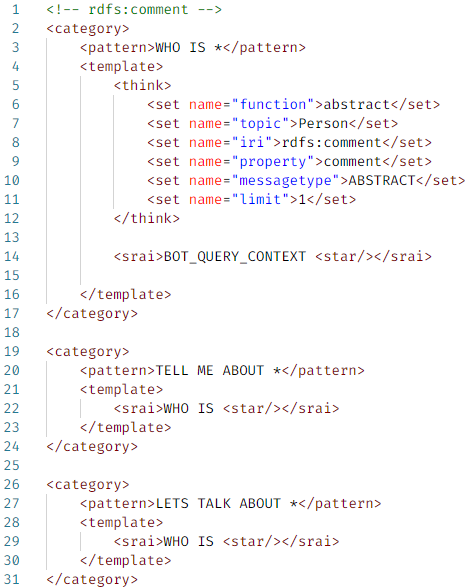
\includegraphics[width=6cm]{aiml-comment}
	\caption{AIML pattern for WHO IS *}
	\label{fig:aiml-comment}
	\subfloat[AIML to decide query context\label{subfig:aiml1}]{{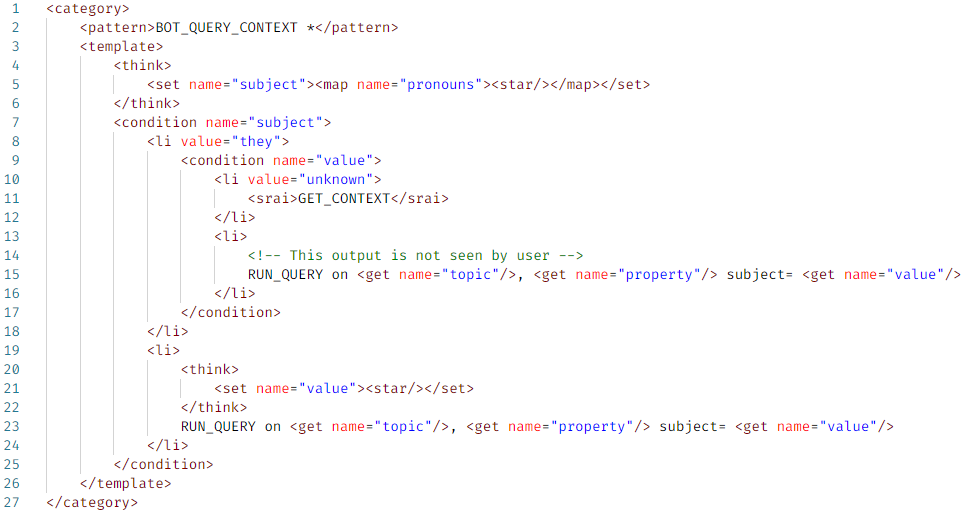
\includegraphics[width=.6\textwidth]{aiml-context} }}%
	\qquad
	\subfloat[AIML to redirect pronoun queries\label{subfig:aiml2}]{{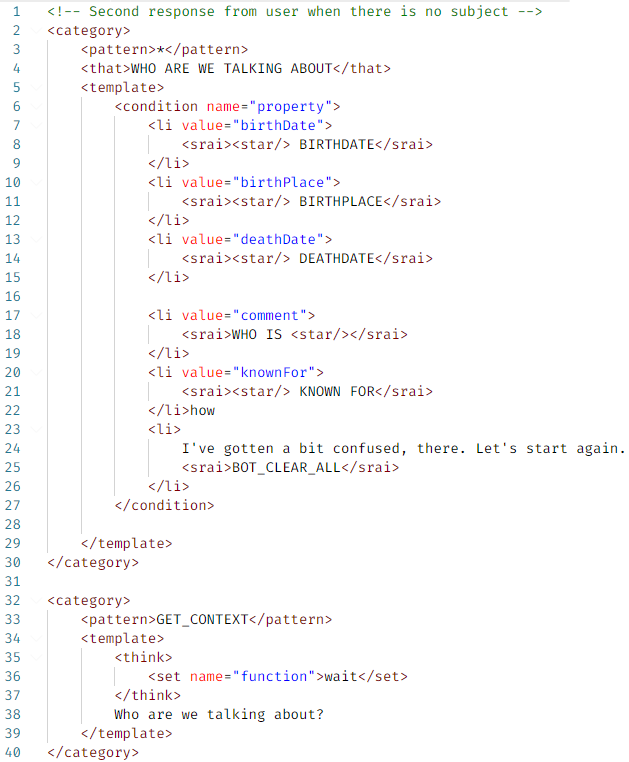
\includegraphics[width=.4\textwidth]{aiml-redirect} }}%
	\caption{AIML logic to handle pronouns}
	\label{fig:aiml-pronouns}
\end{figure}

\newpage
\subsubsection{Query Builder}
We can build a query based on the predicates that we set in the AIML patterns. Most of the simple queries follow a similar pattern to that seen in Figure~\ref{fig:sparql1} - selecting a property given a set of conditions. For these queries we can build a query string, inserting the values provided by the user from the AIML predicates.

In the final system ... UserQuery ... \hilight{continue}

\subsubsection{DBPedia Service}
The role of the \code{DBPedia} class is to execute queries and return a result. This class is divided into a number of methods for each type of query. For example, executing a query about a person in \code{executePersonQuery()} requires different logic to \code{executeAgeQuery()} where further processing has to take place. Each method makes changes to the \code{Message} instance which contains the chatbot's response. The \code{Message} object has a number of attributes relating to the content and information stored in the message. It also has a list of \code{MessageItems}, where a \code{Message} may contain a list of multiple items. The information stored here is processed by the web interface in order to display the information in the correct format, as discussed in the next section.

\subsection{Web Interface}
Spring Boot \cite{springmanual} was used in this project has the web framework, mainly because of its popularity and configurability for web-based Java projects. To initalise this, the required dependencies are added to the project's \code{pom.xml} file. The \code{org.springframework.boot} provides many helper classes for configuring a Spring Boot application.

In order to manage the web application, our \code{WebController} routes requests and manages state. The web application routing is simple, because there are only three mappings to deal with:
\begin{itemize}
	\item GET index: Displays all messages between user and bot
	\item POST submitMessage: User sends a new message to the bot
	\item POST clear: Clears the chat history
\end{itemize}

For displaying the web views, Thymeleaf \footnote{https://www.thymeleaf.org/} is used in this project because it integrates well with Spring, and gives us a lot of flexibility with conditionally styling and displaying elements. Bootstrap \footnote{https://getbootstrap.com/} is also used as a CSS library to homogenize the front-end design, and allow for quickly configuring elements.

The final user interface is shown in Figure~\ref{fig:final-ui}. The layout is simple, with a \code{navbar} element at the top and the main body containing the chat window, which contains the messages sent between the user and the bot. The messages are retrieved from the \code{MessageRepository} by the controller, which are iterated over by the Thymeleaf function in the \code{index.html} page. These messages are conditionally formatted, based on the \code{Sender} attribute of the message. We can see that the larger message is formatted to contain an image and a link - this is based on the \code{MessageType} attribute being equal to \code{ABSTRACT} - this was initially flagged by the bot AIML pattern when the user entered the query `who is alan turing'.

\begin{figure}[h]
	\centering
	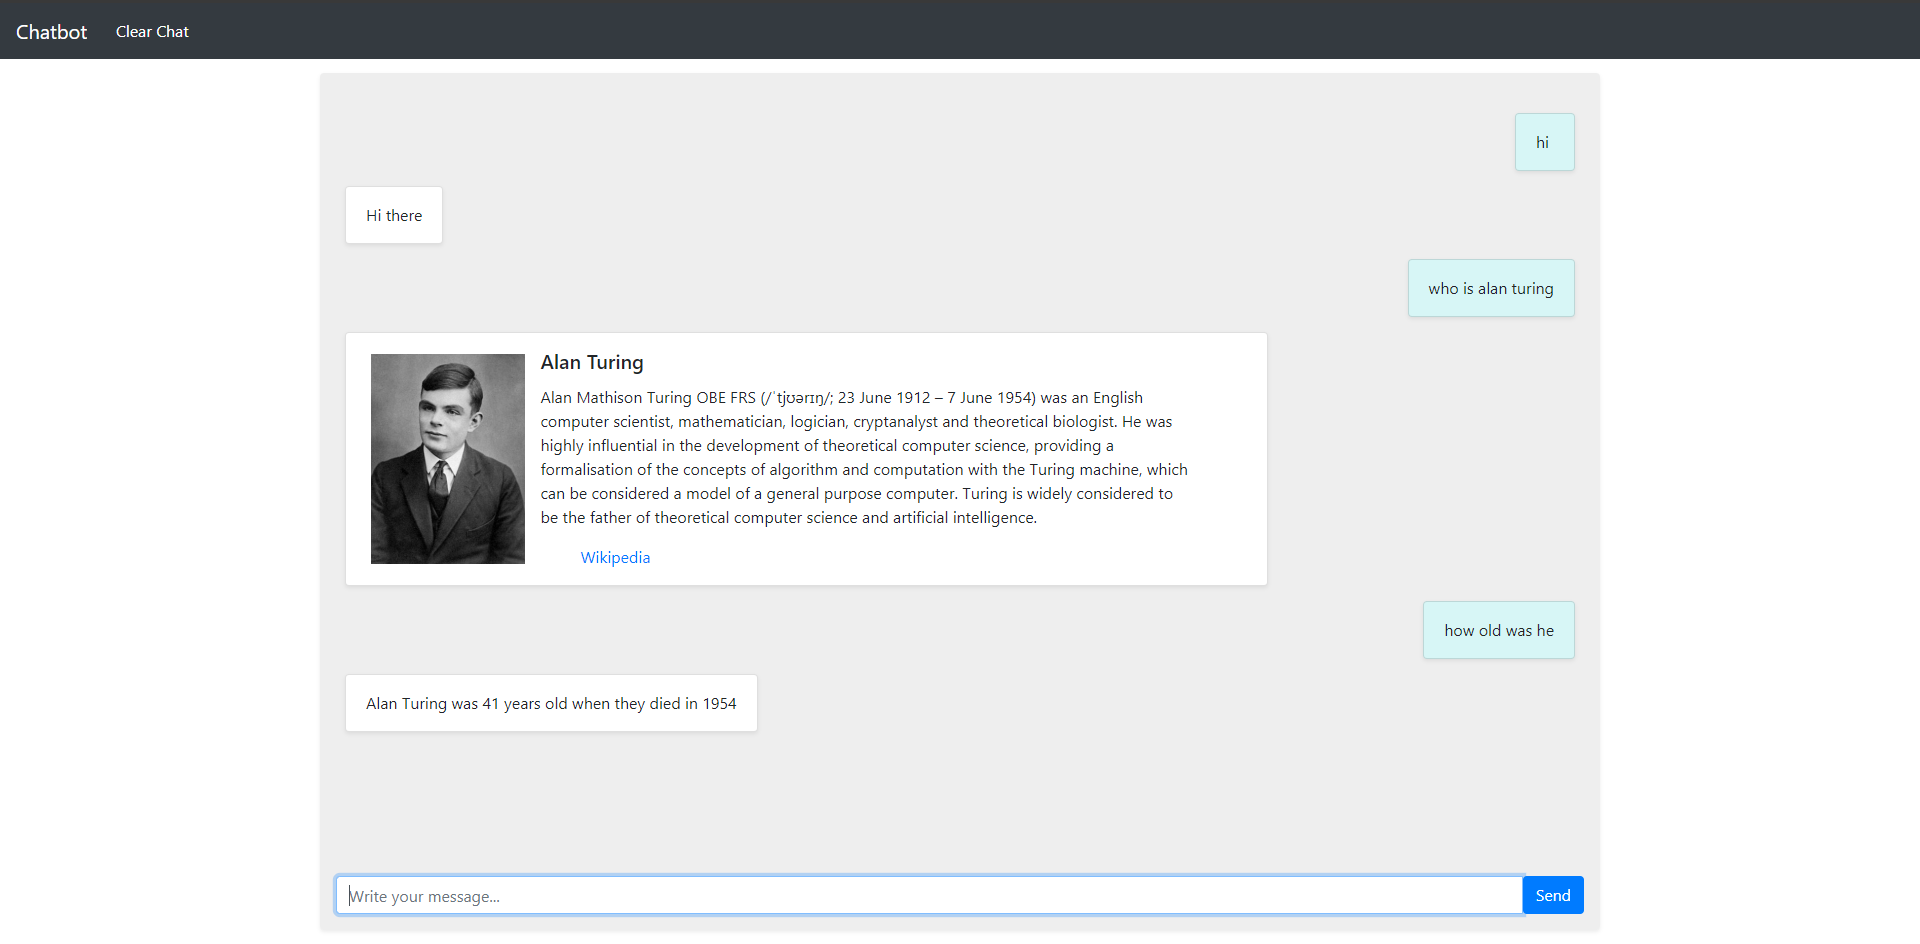
\includegraphics[width=\textwidth]{final-ui}
	\caption{Final UI design}
	\label{fig:final-ui}
\end{figure}

\newpage
\subsection{Hibernate Database}
In order to maintain a conversation history with the chatbot, as well as manage multiple users, a database is required to store messages. However, storing user data has legal and ethical considerations - this is discussed in detail in Chapter~\ref{ch:ethics}. For this implementation, I made a conscious effort to store as little information about the user as possible. Hibernate H2 \footnote{http://www.h2database.com/html/main.html} allows us to persist data in our web application, as well as provide object-relational mapping (ORM) to the database. H2 allows us to create an in-memory database, so that data is not stored and is lost when the application is restarted.

The schema of the database is automatically generated on start-up, based on the Spring \code{Entities} in our application. For this application we have the \code{Message} entity, which stores the content and metadata of each message. We also have the \code{MessageItem} entity, which can form the basis of a \code{LIST} message, where each \code{MessageItem} may have metadata such as a URI. In the \code{Message} entity, we define the relationship between \code{Message} and \code{MessageItem} as \code{OneToMany}, as we can have multiple \code{MessageItems} in a single \code{Message}. The attributes of \code{Message} are shown in Figure~\ref{fig:message}, which shows the tags used to achieve this objective.

\begin{figure}[h]
	\centering
	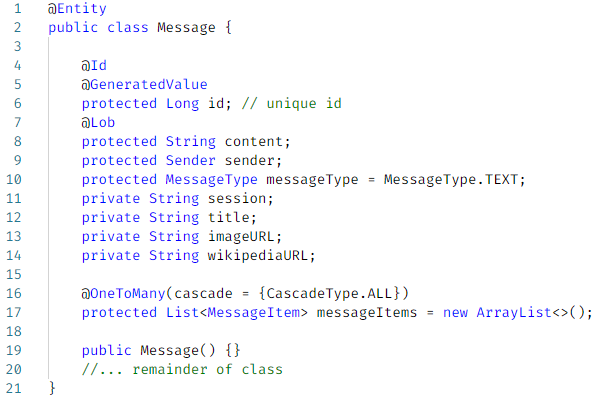
\includegraphics[width=.5\textwidth]{message}
	\caption{Message class}
	\label{fig:message}
\end{figure}


Spring Data can provide CRUD operations (create, read, update, delete) for an ORM using a repository interface; here we are using \code{CrudRepository}. This allows us to easily add messages to the conversation. This interface is provided by the \code{MessageRepository} class - a similar one is required for \code{MessageItemRepository} to provide an interface for the \code{MessageItem} entities. The \code{MessageRepository} interface provides functionality to the \code{WebController}, including adding additional functions such as finding messages by Session ID. The code for this is shown in Figure~\ref{subfig:message}, and is used in Figure~\ref{subfig:webcontroller} to save messages to the database.

\begin{figure}[h]
	\centering
	\subfloat[MessageRepository interface \label{subfig:message}]{{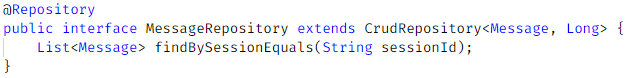
\includegraphics[width=.6\textwidth]{messagerepo} }}%
	\qquad
	\subfloat[WebController logic \label{subfig:webcontroller}]{{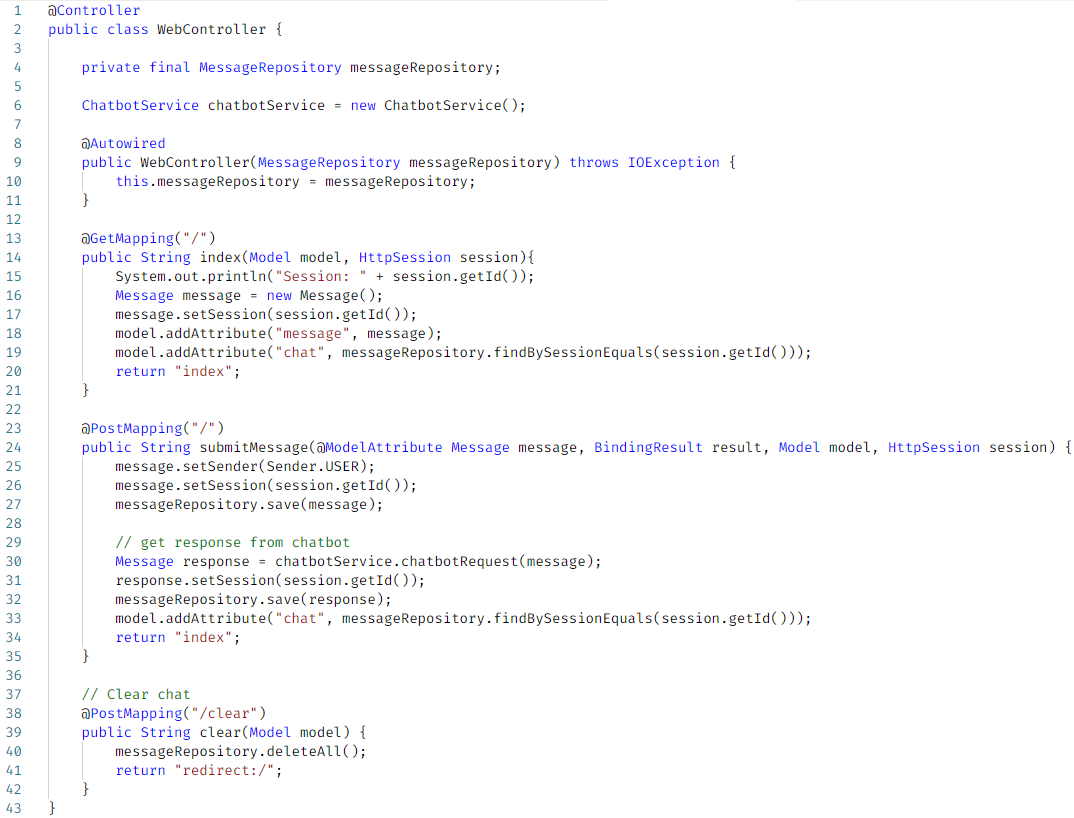
\includegraphics[width=\textwidth]{webcontroller} }}%
	\caption{Controller logic}
	\label{fig:aiml-pronouns}
\end{figure}

\newpage
\section{Challenges}
This section discusses some of the challenges encountered during the implementation of this project. It describes some of the solutions used to overcome these obstacles.

\subsection{Limitations of AIML}
One of the fundamental challenges of using the pattern-based AIML is handling synonyms. I discovered that there are many ways that a particular question can be asked. Furthermore, since the requirements of the system pertain to both Person queries and Country queries, the system must be able to distinguish between the two topics of conversation.

The use of sets and maps was key to solving this problem. In order to `teach' the chatbot what a country is, a set was created named \code{countries.txt} with a list of every country from the DBPedia dataset. These were loaded programatically using a DBPedia query in the \code{ChatbotUtils} class. One issue here was that simply querying a list of all records belonging to \code{dbo:Country} also included every historic kingdom, dominion, dynasty, caliphate, as well as some bizarre outliers - a further discussion of inconsistencies of the dataset is given in Section~\ref{sec:dataset}. Therefore to return useable data, the results had to be filtered to exclude results with a \code{dbo:dissolutionYear}, as well as include countries that included a \code{dbo:Capital}.

The final query used in this utility is given in Figure~\ref{fig:sparqlcountry}. Given a list of all countries, we can then map the country to its Uniform Resource Locator (URI) to easily query that exact country - this is mapped in the file \code{country2dbr.txt}.

\begin{figure}[h]
	\begin{lstlisting}
		SELECT DISTINCT ?country ?name
		WHERE {
		  ?country a dbo:Country.
		  ?country dbo:capital ?capital .
		  ?country rdfs:label ?name 
		  FILTER NOT EXISTS { ?country dbo:dissolutionYear ?yearEnd }
		  FILTER langMatches(lang(?name), 'en')
		} ORDER BY ?country
	\end{lstlisting}
	\caption{SPARQL for listing every country}
	\label{fig:sparqlcountry}
\end{figure}


\subsection{SPARQL Queries}
One of the challenges with querying the DBPedia dataset derives from the requirement for generating lists (requirement F17). While it is trivial to list every actor using a basic query, it is important to give meaningful results to the user. For example, if the user wants a list of actors, we might use the query shown in Figure~. The challenge here is: what order should these results be displayed? If they are displayed alphabetically, as shown in Figure~, the user will not get much use out of those results. The solution here was to use 
\begin{itemize}
	\item Searching
	\item Lists - return order - vrank
\end{itemize}

\subsection{Spring Framework}

\subsection{Dataset Inconsistencies}
\label{sec:dataset}
\begin{itemize}
	\item Actors 
	\item Countries - England displayed as a dbo:MusicalArtist
\end{itemize}


\section{Conclusion}



	\chapter{Testing}
\label{ch:testing}
\section{Introduction}
\newpage

\begin{landscape}
	\section{Requirements Testing}
	\begin{tabularx}{\hsize}{lXXXr}
		\toprule
		ID & Name & Expected Output & Evidence & Success? \\
		\midrule
		F1 & User Interaction 
		& A page should display to allow the user to interact with the bot
		& 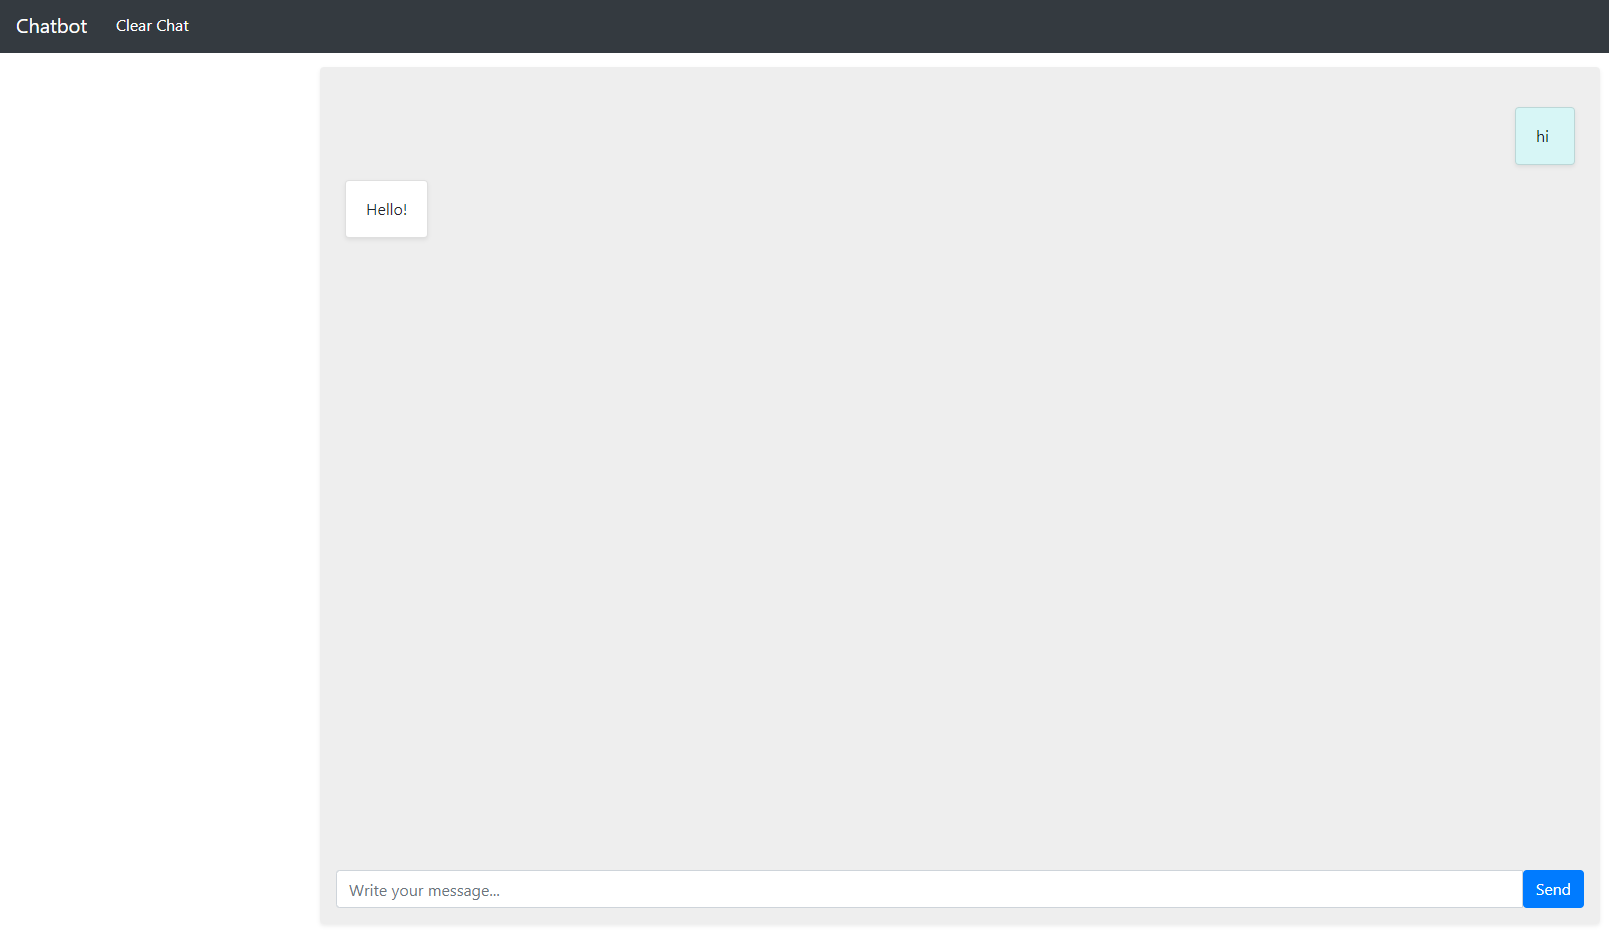
\includegraphics[width=8cm]{tests/f1} & Yes \\
		\midrule
		F2 & Browser Access
		& The user should be able to access the system via a browser
		& 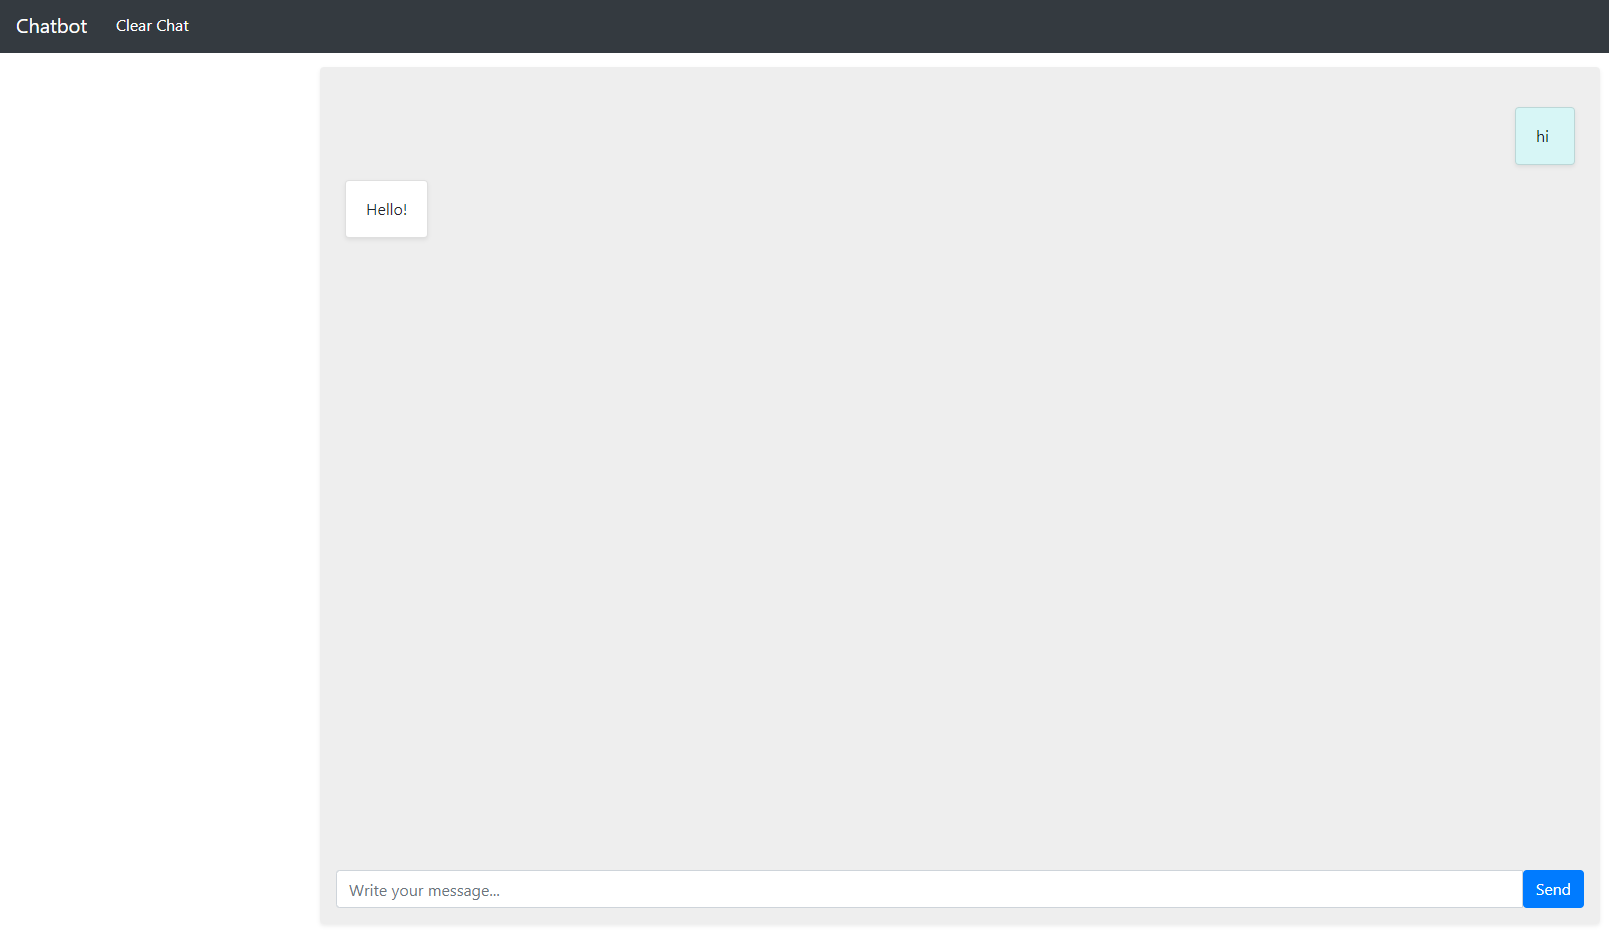
\includegraphics[width=8cm]{tests/f1} & Yes \\
		\midrule
		F3 & User Input
		& The user should be enter queries to the bot using a textbox input
		& 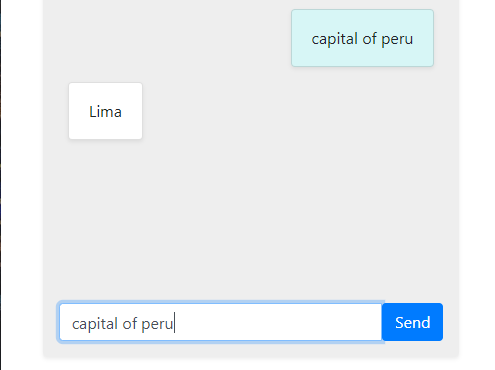
\includegraphics[width=8cm]{tests/f3} & Yes \\
		\bottomrule
		F4 & Responses on Page
		& The should see the chatbot response on the web page
		& 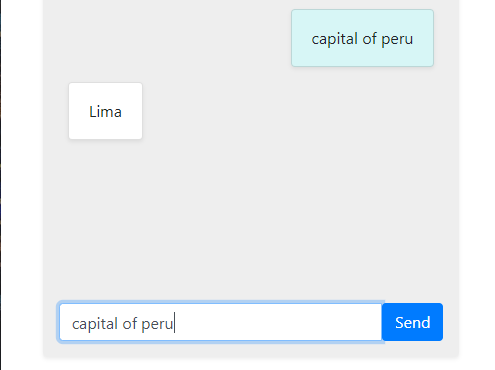
\includegraphics[width=8cm]{tests/f3} & Yes \\
		\bottomrule
		F5 & Conversation History
		& The should see the whole conversation with the bot on the page
		& 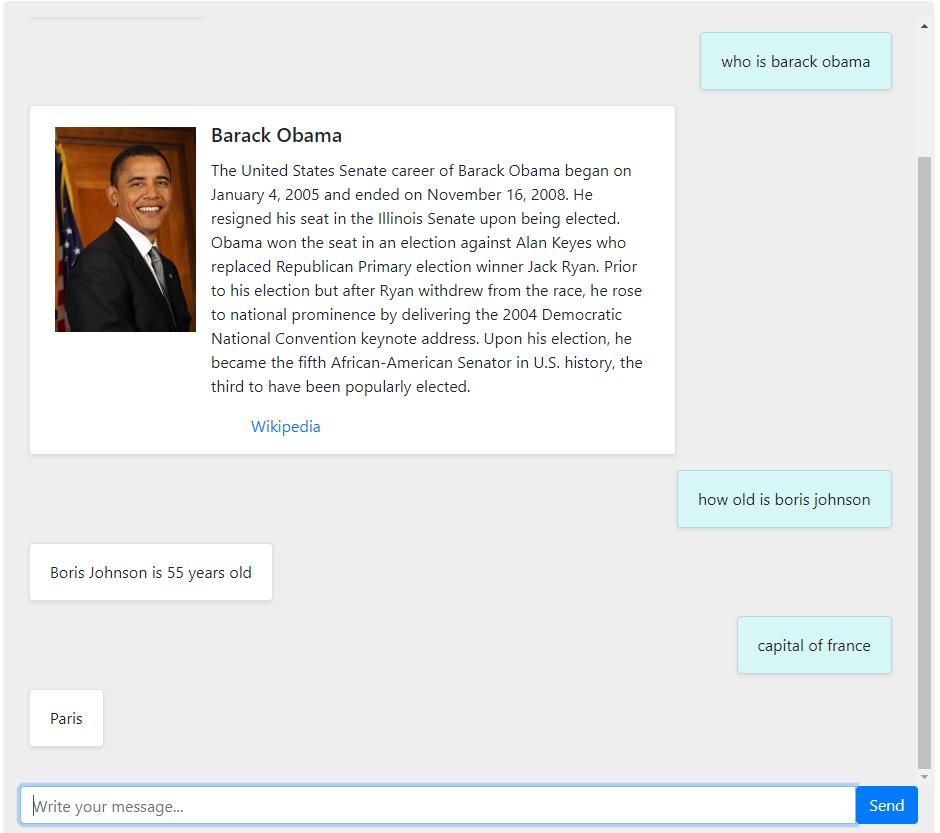
\includegraphics[width=8cm]{tests/f5} & Yes \\
		\bottomrule
		F6 & Person Description Query
		& The user should be able to ask a query about who a person is\newline - 'WHO IS *' and receive a description of that person
		& 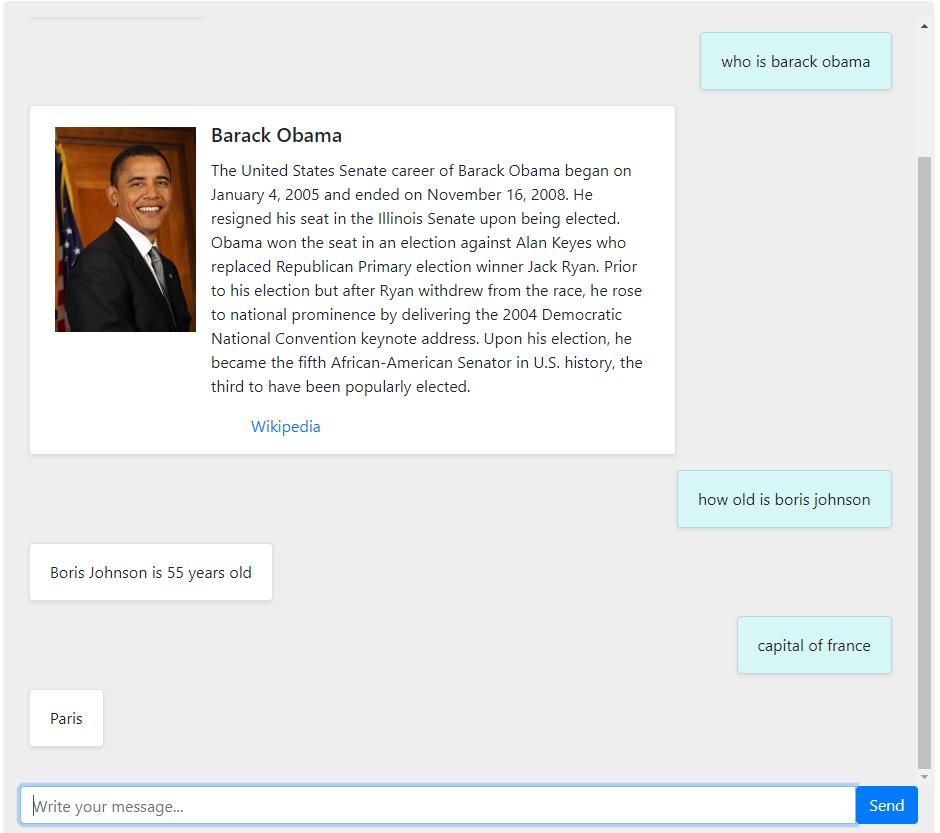
\includegraphics[width=8cm]{tests/f5} & Yes \\
		\bottomrule
		F7 & Person Birthdate Query
		& The user should be able to ask a query about when a person was born\newline - 'WHEN WAS * BORN' and see their birth date
		& 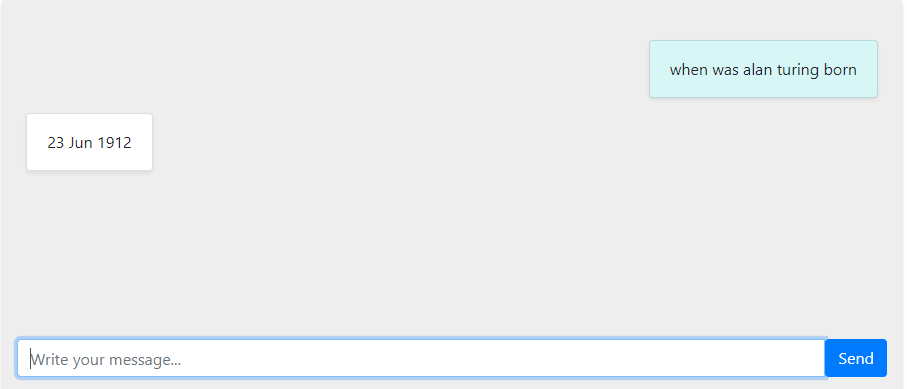
\includegraphics[width=8cm]{tests/f7} & Yes \\
		\bottomrule
		F8 & Person Age Query
		& The user should be able to ask a query about a person's age\newline - 'HOW OLD IS *' and see their age
		& 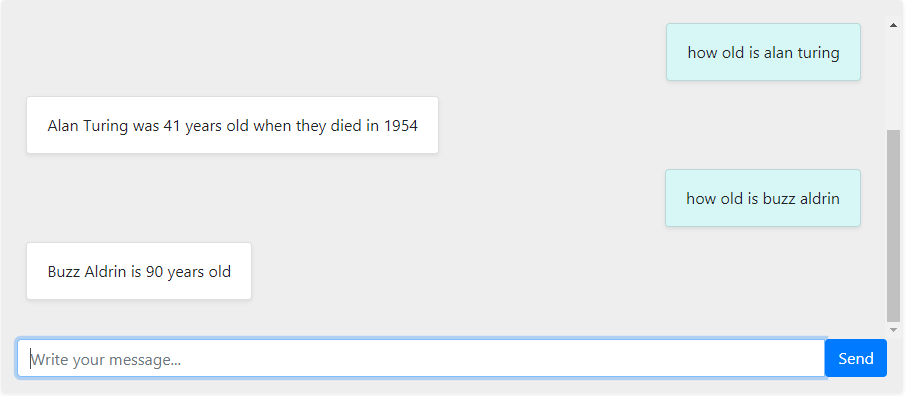
\includegraphics[width=8cm]{tests/f8} & Yes \\
		\bottomrule
		F9 & Person Birthplace Query
		& The user should be able to ask a query about where a person was born\newline - 'WHEN WAS * BORN' and see their birthplace
		& 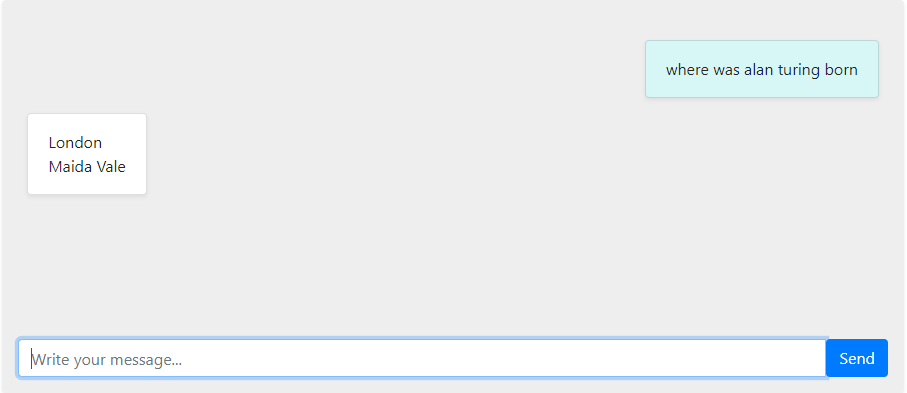
\includegraphics[width=8cm]{tests/f9} & Yes \\
		\bottomrule
		F10 & Person Death Date query
		& The user should be able to ask a query about when a person died\newline - 'WHEN DID * DIE' and see their death date
		& 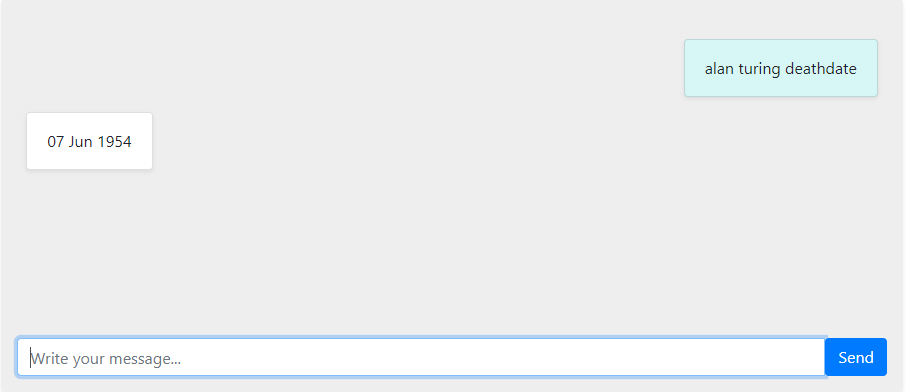
\includegraphics[width=8cm]{tests/f10} & Yes \\
		\bottomrule
		F11 & Person Known For Query
		& The user should be able to ask a query about what a person is known for\newline - 'WHAT IS * KNOWN FOR' and see what they are known for
		& 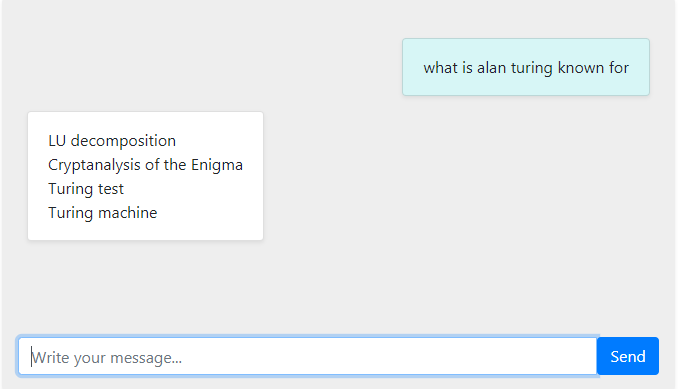
\includegraphics[width=8cm]{tests/f11} & Yes \\
		\bottomrule
		F12 & Person Photo Query
		& The user should be able to ask for a photo of a person\newline - 'WHAT DOES * LOOK LIKE' and see a photo of the person
		& 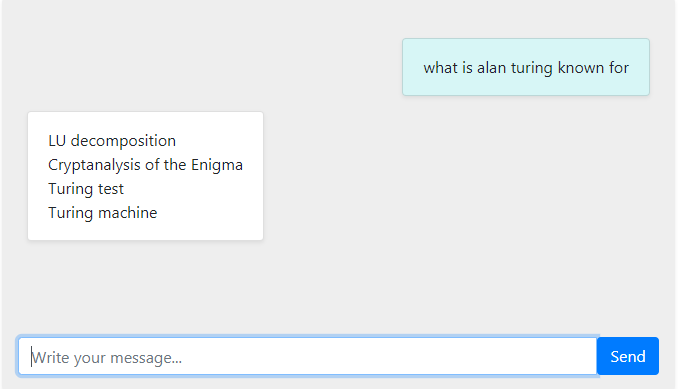
\includegraphics[width=8cm]{tests/f11} & Yes \\
		\bottomrule
		F13 & Person Wikipedia Link Query
		& The user should be able to ask for the link to a person's Wikipedia page\newline - '* WIKIPEDIA PAGE' and receive a link to their page
		& 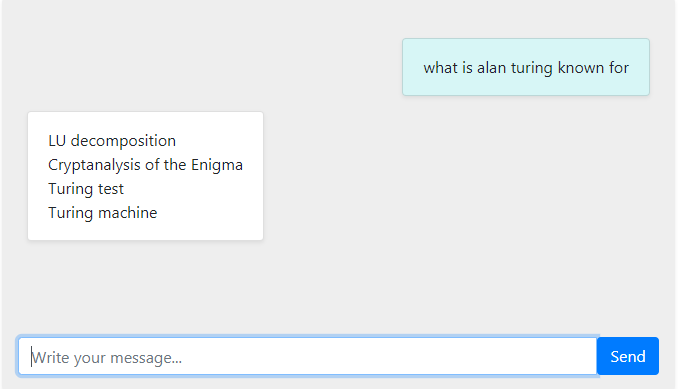
\includegraphics[width=8cm]{tests/f11} & Yes \\
		\bottomrule
		F14 & Country Description Query
		& The user should be able to ask about a country\newline - '[COUNTRY]' and see a description of that country
		& 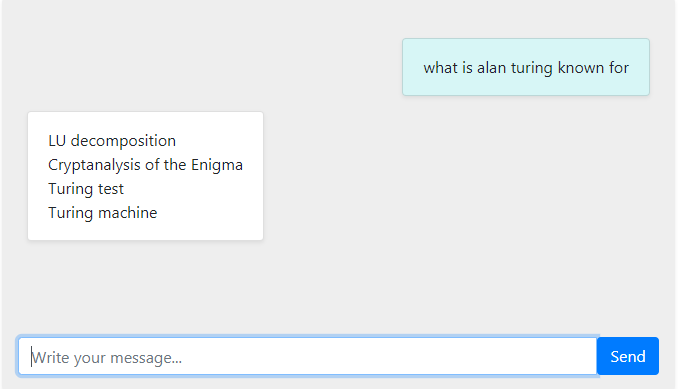
\includegraphics[width=8cm]{tests/f11} & Yes \\
		\bottomrule
		F15 & Country Population Query
		& The user should be able to ask about a country\newline - '[COUNTRY] POPULATION' and see the population of that country
		& 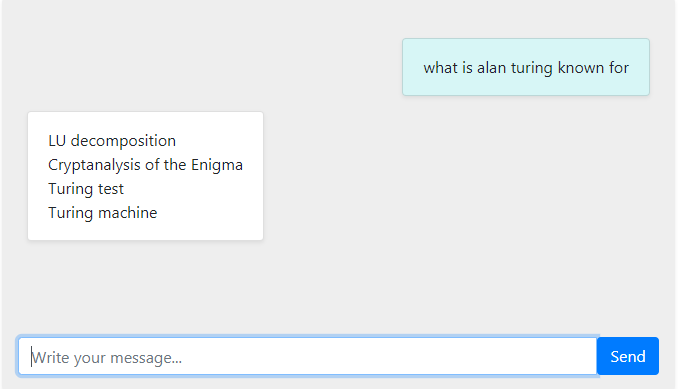
\includegraphics[width=8cm]{tests/f11} & Yes \\
		\bottomrule
		F16 & Country Capital Query
		& The user should be able to ask for the capital of a country\newline - 'CAPITAL OF [COUNTRY]' and see the capital of that country
		& 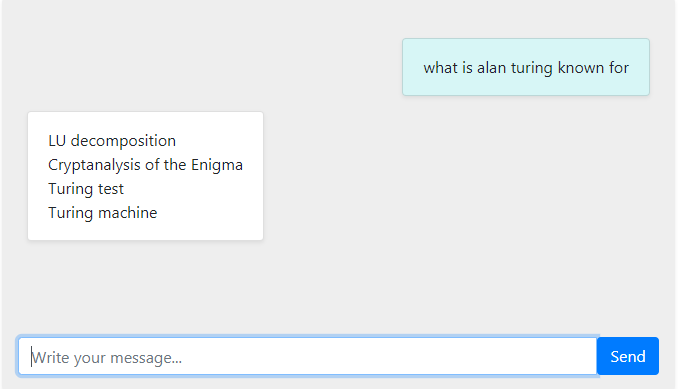
\includegraphics[width=8cm]{tests/f11} & Yes \\
		\bottomrule
		F17 & Person List Query
		& The user should be able to ask for lists of people\newline - 'LIST OF ACTORS' - and see a list of actors 
		& 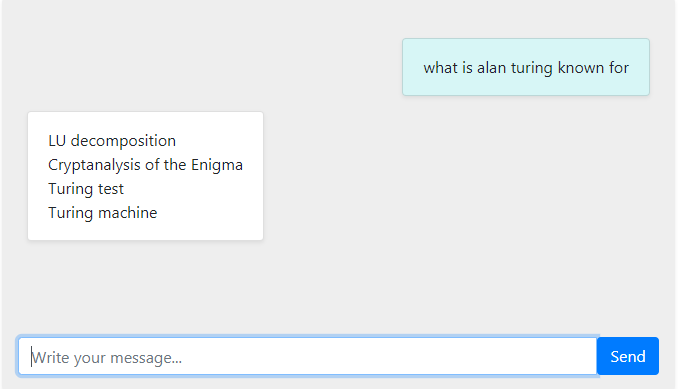
\includegraphics[width=8cm]{tests/f11} & Yes \\
		\bottomrule
		F18 & Person AND Query
		& The user should be able to combine queries\newline - 'LIST OF ACTORS BORN IN 1990 AND BORN IN LONDON'\newline and see a list matching that conditional query
		& 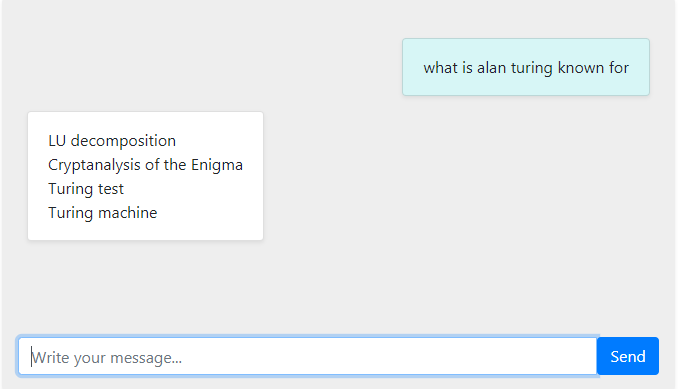
\includegraphics[width=8cm]{tests/f11} & Yes \\
		\bottomrule
		F19 & Context-aware Conversation
		& The user should be able to continue from previous queries using pronouns\newline e.g. 'WHEN WAS HE BORN' and the chatbot should maintain the context of the query
		& 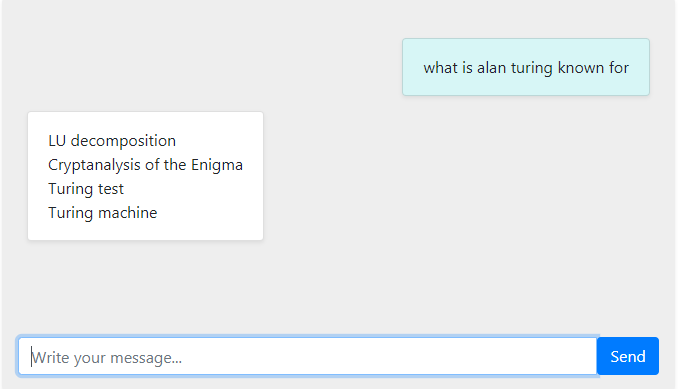
\includegraphics[width=8cm]{tests/f11} & Yes \\
		\bottomrule
		F20 & Chatbot Greeting
		& The chatbot should be able to greet the user
		& 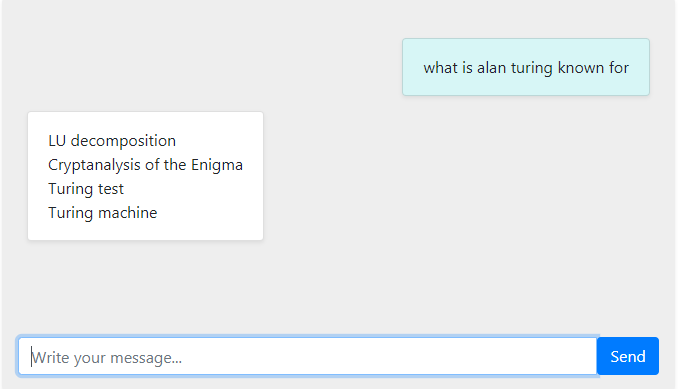
\includegraphics[width=8cm]{tests/f11} & Yes \\
		\bottomrule
		F21 & Chatbot Examples
		& The chatbot should display a list of example queries\newline when asked 'EXAMPLES' or 'WHAT CAN YOU DO'
		& 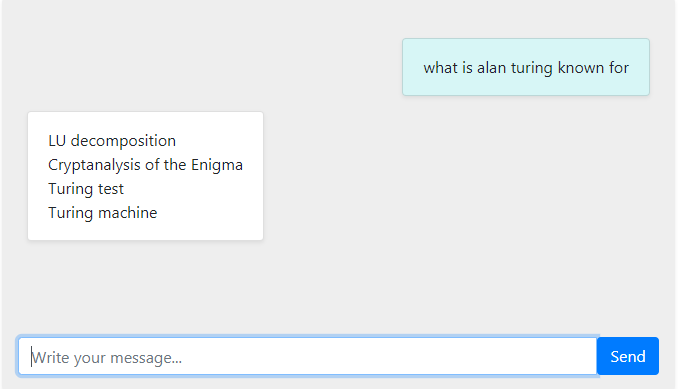
\includegraphics[width=8cm]{tests/f11} & Yes \\
		\bottomrule
		F22 & Chatbot Help
		& The user should be able to receive help from the chatbot\newline on how to use it when asked 'HELP'
		& 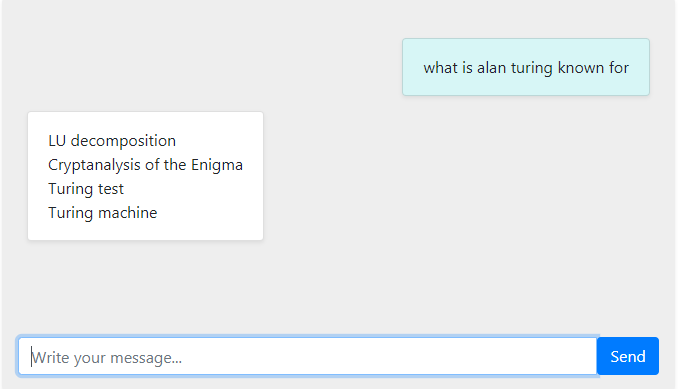
\includegraphics[width=8cm]{tests/f11} & Yes \\
		\bottomrule
		P1 & Web page loads in 5 seconds
		& 
		& 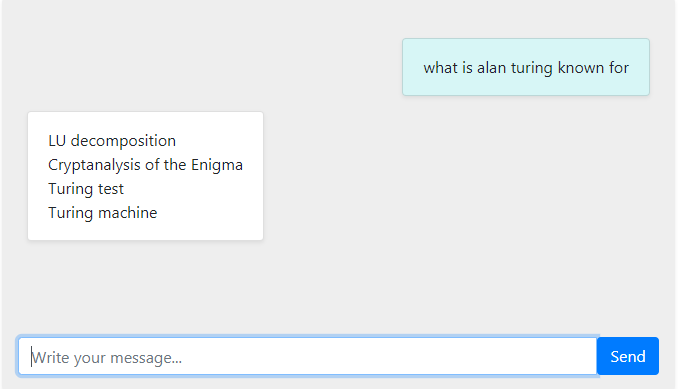
\includegraphics[width=8cm]{tests/f11} & Yes \\
		\bottomrule
		P2 & Chatbot responds in 5 seconds
		& 
		& 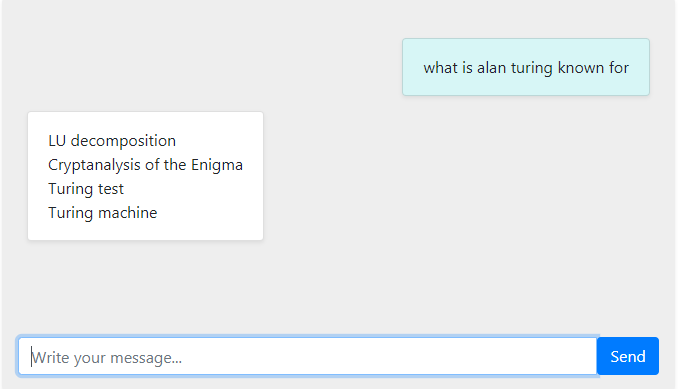
\includegraphics[width=8cm]{tests/f11} & Yes \\
		\bottomrule
		P3 & Application functions without failure
		& 
		& 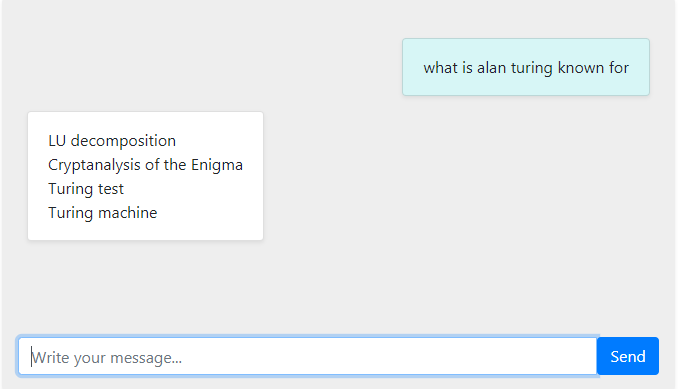
\includegraphics[width=8cm]{tests/f11} & Yes \\
		\bottomrule
		P4 & Any errors are logs and the user is informed
		& 
		& 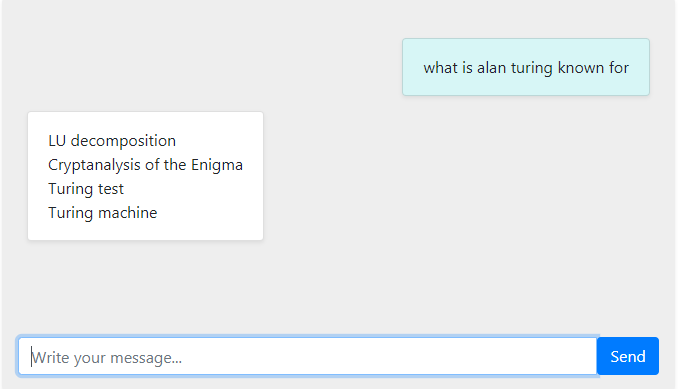
\includegraphics[width=8cm]{tests/f11} & Yes \\
		\bottomrule
		%\caption{Requirements testing and evidence}
		%\label{tab:testreq}
	\end{tabularx}
\end{landscape}


\newpage
\section{Unit Testing}
\section{User Acceptance Testing}
\section{Conclusion}
	\chapter{Evaluation}
	\chapter{Conclusion}
\section{Overview}
\section{Conclusions}
\section{Future Work}
\section{Final Statement}
	
	% back matter
	\bibliography{references}

	\appendix
	\addcontentsline{toc}{chapter}{Appendices}
	\chapter{Wikimedia API}
\label{ch:wikimedia}
The following Figure~\ref{fig:wiki} shows a fragment of the response when running a query using the MediaWiki API \cite{mediawiki}. The result has been truncated, and is the response from the query

\begin{lstlisting}
	https://en.wikipedia.org/w/api.php?action=query&prop=revisions
		&rvprop=content&rvsection=0&titles=Tim%20Berners-Lee
\end{lstlisting}

\begin{figure}[h]
	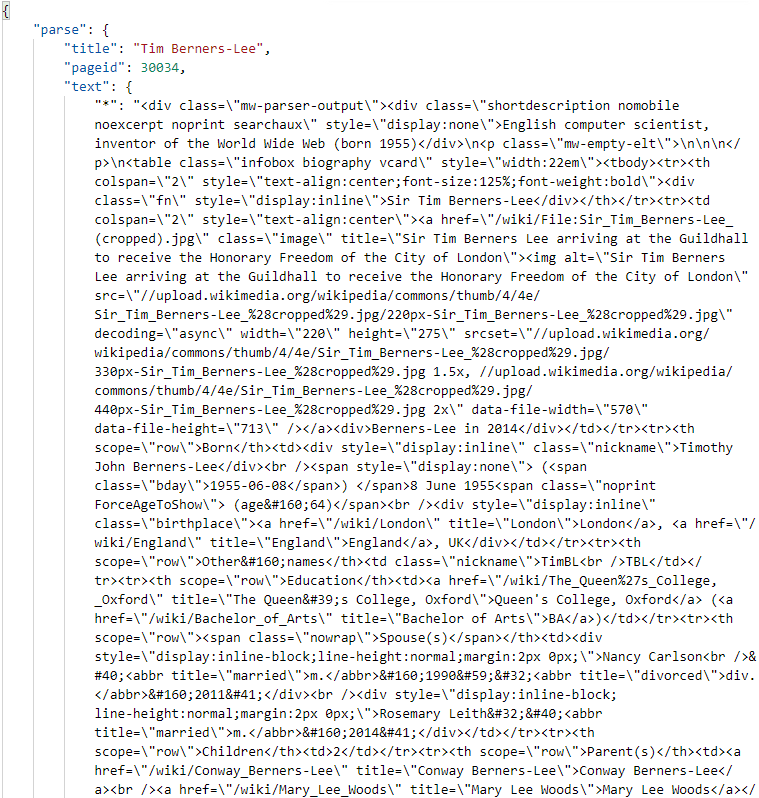
\includegraphics[width=\textwidth,height=\textheight,keepaspectratio]{wikimedia}
	\caption{A JSON response excerpt from a MediaWiki query.}
	\label{fig:wiki}
\end{figure}

\end{document}